%=== How to use:
%   \confvertrue, \plainverfalse = 2 column IEEE version
%   \confverfalse, \plainverfalse = 1 column IEEE draft version
%   \plainvertrue = our plain version

\newif\ifconfver
%\confverfalse      %declaring conference version false
\confvertrue        %declaring conference version true

\newif\ifonecoltab
\onecoltabtrue        % declaring one column version table size true
%\onecoltabfalse

\newif\ifplainver  %declare a plain version
%\plainvertrue
%\plainverfalse

\ifplainver
    \confverfalse                         %automatically disable conf. version argument if it's plain
\fi

\ifconfver
     \documentclass[10pt,journal]{IEEEtran}
\else
    \ifplainver
        \documentclass[11pt]{article}
        \usepackage{fullpage}
    \else
        \documentclass[12pt,draftcls,onecolumn]{IEEEtran}
    \fi
\fi




\usepackage{calc,amsfonts,amssymb,amsmath,bm,url,color,theorem,graphicx,cite,epstopdf,nicefrac}
\usepackage{psfrag,subfigure,float}
\usepackage[algoruled,linesnumbered]{algorithm2e}
\usepackage{multirow}
%\usepackage{algorithm}
%\usepackage{algorithmic}
\usepackage[normalem]{ulem}

%--- define color
\definecolor{orange}{RGB}{255,107,0}
\def\blue{\color{blue}}
\def\red{\color{red}}
\def\orange{\color{orange}}
\def\green{\color{green}}

%--- defining the theorem and stuff

\newtheorem{Fact}{Fact}
\newtheorem{Lemma}{Lemma}
\newtheorem{Prop}{Proposition}
\newtheorem{Theorem}{Theorem}
\newtheorem{Def}{Definition}
\newtheorem{Corollary}{Corollary}
\newtheorem{Property}{Property}
\newtheorem{Observation}{Observation}
\theorembodyfont{\rmfamily}
\newtheorem{Exa}{Example}
\newtheorem{Assumption}{Assumption}
\newtheorem{Remark}{Remark}


%make sure to keep this for convenience later
\newcommand\bd{\ensuremath{{\rm bd}}}
\newcommand\inte{\ensuremath{{\rm int}}}
%---- vectors -----------------
\newcommand{\vct}{\bm{t}}
\newcommand{\vcx}{\bm{x}}
%---- sets --------------------
\newcommand{\setB}{\mathcal{B}}
\newcommand{\setR}{\mathcal{R}}
\newcommand{\setW}{\mathcal{W}}
\newcommand{\Rbb}{\mathbb{R}}
\newcommand{\MVES}{\mathsf{MVES}}





\newcommand{\W}{\boldsymbol{W}}
\newcommand{\G}{\boldsymbol{G}}
\newcommand{\Q}{\boldsymbol{Q}}
\newcommand{\X}{\boldsymbol{X}}
\newcommand{\C}{\boldsymbol{C}}
\newcommand{\E}{\boldsymbol{E}}
\newcommand{\U}{\boldsymbol{U}}
\newcommand{\K}{\mathcal{K}}
\newcommand{\one}{\boldsymbol{1}}
\newcommand{\M}{\boldsymbol{M}}
\newcommand{\A}{\boldsymbol{A}}
\newcommand{\B}{\boldsymbol{B}}
\newcommand{\x}{\boldsymbol{x}}
\newcommand{\m}{\boldsymbol{m}}
\renewcommand{\a}{\boldsymbol{a}}
\renewcommand{\th}{\boldsymbol{\theta}}

%%%%%%%%%%%%%%%%%%%%%%%%%%%%%%%%%%%%%%%%%%%%%%%%%%%%%%%%%%%%%%%%%%%%%%%%%%%%%%%
% From Nikos: reminder command:
\newcommand{\reminder}[1]{ \color{blue} [[[ \marginpar{\mbox{\color{blue} ${\bf <==}$ \color{black}}} #1 ]]] \color{black}}
%\newcommand{\reminder}[1]{} % do not show reminders
%%%%%%%%%%%%%%%%%%%%%%%%%%%%%%%%%%%%%%%%%%%%%%%%%%%%%%%%%%%%%%%%%%%%%%%%%%%%%%%

% correct bad hyphenation here
\hyphenation{op-tical net-works semi-conduc-tor}


\begin{document}



%--- I do things quite strangely here to accommodate three style modes.
%--- input title and abstract here; it applies to all modes
%--- it's too complex to do authors or they are input for each mode
\newcommand{\papertitle}{
%Robust Volume Minimization-Based Matrix Factorization for Remote Sensing and Document Clustering
Scalable and Flexible Multiview  MAX-VAR Canonical Correlation Analysis
}

\newcommand{\paperabstract}{
This paper considers generalized (multiview) canonical correlation analysis (GCCA) for large-scale datasets.
%A memory-efficient and computationally lightweight algorithmic framework is proposed for the classic MAX-VAR GCCA formulation as well as its variants.
GCCA is gaining renewed interest in various applications such as speech processing and natural language processing. The classic MAX-VAR GCCA problem can be solved optimally via eigen-decomposition of a matrix that compounds the (whitened) correlation matrices of the views. 
However, this route can easily lead to memory explosion and a heavy computational burden when the size of the views becomes large. 
In addition, it was unclear how to promote pre-specified structure (e.g. sparsity) on the canonical components sought, while structured component analysis is often desired in data analytics.
In this work, we propose an alternating optimization (AO)-based algorithm to handle large-scale MAX-VAR GCCA as well as its variants that impose structure on the canonical components.
The algorithm avoids instantiating the correlation matrices of the views and thus can achieve substantial saving in memory. It also maintains data sparsity, which can be exploited to alleviate the computational burden. 
Consequently, the proposed algorithm is highly scalable and flexible in handling a variety of regularizations.
Convergence properties of the proposed algorithm are carefully studied:
It is shown to converge to a critical point at least at a sublinear convergence rate using a certain class of (possibly non-smooth) structure-promoting regularizations. If the original MAX-VAR problem is considered, we improve the convergence rate to a linear one. Simulations and large-scale word embedding tasks are employed to showcase the effectiveness of the proposed algorithm.
}

%--------

\ifplainver

    \date{\today}

    \title{\papertitle}

    \author{
    Xiao Fu$^\ast$, Kejun Huang$^\ast$, Mingyi Hong	$^\ddag$, Nicholas D. Sidiropoulos$^\ast$, and Anthony Man-Cho So$^\dag$
    \\ ~ \\
		$^\ast$Department of Electrical and Computer Engineering, University of Minnesota,\\
		Minneapolis, 55455, MN, United States\\
		Email: (xfu,huang663,nikos)@umn.edu
	  \\~\\
	$^\ddag$Department of Industrial and Manufacturing Systems Engineering, Iowa State University\\
	Ames, Iowa 50011, (515) 294-4111,\\
	Email: mingyi@iastate.edu
	 \\ ~ \\
    $^\dag$Department of Systems Engineering and Engineering Management\\ The Chinese University of Hong Kong, \\
	Shatin, N.T., Hong Kong \\
	Email: manchoso@se.cuhk.edu.hk 
	\\
    }

    \maketitle
	

    \begin{abstract}
    \paperabstract
    \end{abstract}

\else
    \title{\papertitle}

    \ifconfver \else {\linespread{1.1} \rm \fi

   \author{Xiao Fu, Kejun Huang, Mingyi Hong,  Nicholas D. Sidiropoulos, and Anthony M.-C. So
\thanks{X. Fu, K. Huang and N.D. Sidiropoulos are with the Department of Electrical and Computer Engineering, University of Minnesota, Minneapolis, MN55455, e-mail (xfu,huang663,nikos)@umn.edu.
M. Hong is with Department of Industrial and Manufacturing Systems Engineering, Iowa State University,	Ames, Iowa 50011, (515) 294-4111, Email: mingyi@iastate.edu.
Anthony M.-C. So is with the Department of Systems Engineering and Engineering Management, The Chinese University of Hong Kong, Shatin, N.T., Hong Kong, Email: manchoso@se.cuhk.edu.hk 
}
}

    \maketitle

    \ifconfver \else
        \begin{center} \vspace*{-2\baselineskip}
        %11th Revision, \today \\[2\baselineskip]
        \end{center}
    \fi

    \begin{abstract}
    \paperabstract
    \end{abstract}

    \begin{keywords}\vspace{-0.0cm}
        Canonical correlation analysis, multiview, word embedding, optimization, scalability, feature selection
    \end{keywords}

    \ifconfver \else \IEEEpeerreviewmaketitle} \fi

 \fi

\ifconfver \else
    \ifplainver \else
        \newpage
\fi \fi
%---------------------------------------------------------------------------


  
	

%---------------------------------------------------------------------------
\section{Introduction}
Canonical Correlation Analysis (CCA) \cite{hardoon2004canonical} produces low dimensional representations by finding common structure of two or more views corresponding to the same entities.
A view contains high-dimensional representations of the entities in some domain -- e.g., the text and audio representations corresponding to a given word can be considered as different views of this word.
CCA is able to deal with views that have different dimensions, and this flexibility is very useful in data fusion, where one is interested in integrating information gathered from different domains.
Multiview analysis finds numerous applications in signal processing and machine learning, such as 
blind source separation \cite{li2009joint,bertrand2015distributed}, direction-of-arrival estimation \cite{wu1994music}, wireless channel equalization \cite{dogandzic2002finite}, regression \cite{kakade2007multi}, clustering \cite{chaudhuri2009multi}, speech modeling and recognition \cite{arora2014multi,wang2015acoustic}, and word embedding \cite{rastogimultiview}, to name a few.
Classical CCA was derived for the two-view case, but Generalized Canonical Correlation Analysis (GCCA) that aims at handling more than two views has a long history as well \cite{carroll1968generalization}. 
A typical application of GCCA, namely, multi-language word embedding, is shown in  Fig.~\ref{fig:motivation}.

%A typical application of GCCA is word embedding in natural language processing, where the vocabularies from different languages can be considered as multiple views of the same terms.
%Word embedding seeks low-dimensional representations of the terms that are well-aligned with human judgment, and applying GCCA to integrate multiple languages was shown to yield better embedding results relative to single-view analyses such as principle component analysis (PCA) \cite{rastogimultiview}.

\begin{figure}[t]
\centering
{\includegraphics[width=.95\linewidth]{CCA_motivation.pdf}
\caption{Word embedding seeks low-dimensional representations of the entities that are well-aligned with human judgment. Different language data (i.e., ${\bm X}_1$-$\X_3$) can be considered as different views / feature spaces of the same entities. Applying GCCA to integrate multiple languages was shown to yield better embedding results relative to single-view analyses such as principle component analysis (PCA) \cite{rastogimultiview}.
}
\label{fig:motivation}}
\end{figure}


Computationally, GCCA poses interesting and challenging optimization problems.
Unlike the two-view case that admits an algebraically simple solution (via eigen-decomposition),
GCCA is in general not easily solvable.
Many prior works considered the GCCA problem with different cost functions \cite{carroll1968generalization,kettenring1971canonical}, while the proposed algorithms often can only extract a single canonical component and then find others through a deflation process, which is known to suffer from error propagation.
%Convergence properties of the GCCA algorithms are also largely under-investigated, since
%the GCCA formulations often involve non-convex constraints (e.g., manifold constraints) that complicate analysis.
CCA and GCCA can also pose serious scalability challenges,
since they involve auto- and cross-correlations of different views and a whitening stage \cite{ma2015finding}.
These procedures can easily lead to memory explosion and require a large number of flops for computation.
They also destroy the sparsity of the data, which is usually what one relies upon to deal with large-scale problems.
In recent years, effort has been spent on solving these scalability issues, but the focus is mostly on the two-view case \cite{ma2015finding,sun2011canonical,lu2014large}.



Among all different formulations of GCCA, there is a particular one that admits a conceptually simple solution, the so-called MAX-VAR GCCA \cite{carroll1968generalization,van2006generalized,kettenring1971canonical}.
MAX-VAR GCCA was first proposed in \cite{carroll1968generalization}, and its solution amounts to finding the `directions' aligned to those exhibiting maximum variance for a matrix aggregated from the (whitened) auto-correlations of the views.
It can also be viewed as a problem of enforcing {\em identical} latent representations of different views as opposed to highly correlated ones, which is the more general goal of (G)CCA.
The merit of MAX-VAR GCCA is that it can be solved via eigen-decomposition and finds all the canonical components simultaneously (i.e., no deflation is involved).
In practice, MAX-VAR GCCA also demonstrates promising performance in various applications such as word embedding \cite{rastogimultiview} and speech recognition \cite{arora2014multi}.
On the other hand, MAX-VAR GCCA has the same scalability problem as the other GCCA formulations:
It involves correlation matrices of different views and their inverses, which is prohibitive to even instantiate when the data dimension is large.
The work in \cite{rastogimultiview} provided a pragmatic way to circumvent this difficulty: PCA was first applied to each view to reduce the rank of the views,
and then MAX-VAR GCCA was applied to the rank-truncated views. Such a procedure significantly reduces
the number of parameters for characterizing the views and is feasible in terms of memory. However, truncating the rank of the views is prone to information loss, and thus leads to performance degradation.

Besides the basic (G)CCA formulations, \emph{structured} (G)CCA \cite{hardoon2011sparse} that
seeks canonical components with pre-specified structure is often considered in applications.
For example, sparse CCA is desired in data analytics for the purpose of discarding outlying or irrelevant features when performing CCA \cite{witten2009penalized,chen2012structured,witten2009extensions}.
In multi-lingual word embedding \cite{faruqui2014improving,sun2011canonical,rastogimultiview}, for example, it is known that there are many outlying features (i.e., outlying columns in $\X_i$ in Fig.~\ref{fig:motivation}), known as ``stop words''. In brain activation analysis, it is also believed that many voxels are irrelevant and should be somehow discarded \cite{rustandi2009integrating,mitchell2008predicting}. Gene analysis is another example \cite{witten2009penalized,chen2012structured,witten2009extensions}.
Ideally, CCA seeks a few highly correlated latent components, and so it should naturally be able to identify and down-weight irrelevant features automatically. In practice, however, this ability is often impaired when correlations cannot be reliably estimated, when one only has access to relatively few and/or very noisy samples, or when there is model mismatch due to bad preprocessing (e.g., registration). In those cases, performing feature selection jointly with (G)CCA is well-motivated. However, introducing structure regularizations on the sought canonical components makes the optimization problem even harder, since many regularizers are non-differentiable.

\bigskip

\noindent
{\bf Contributions}
In this work, 
our goal is to provide a scalable and flexible algorithmic framework for dealing with
the MAX-VAR GCCA problem and its variants with structure-promoting regularizers.
Instead of truncating the rank of the views as in \cite{rastogimultiview}, we keep the data \emph{intact} and devise a scalable algorithmic framework to handle the formulated problem.
Specifically, our idea is to deal with problem using a two-block alternating optimization (AO) algorithm.
Under the AO framework, the proposed algorithm alternates between a regularized least squares subproblem and an orthogonality-constrained subproblem.
The merit of this framework is that correlation matrices of the views never need to be explicitly instantiated, and the inversion procedure is avoided. 
Consequently, the algorithm consumes significantly less memory compared to that required by the original solution using eigen-decomposition.
In addition, the proposed algorithmi can easily handle
different structure-promoting regularizers without increasing memory and computational costs, including the feature-selective regularizers that we
are mainly interested in.

Convergence properties of the algorithm are also carefully studied:
We first show that the proposed algorithm \emph{globally} converges to a Karush-Kuhn-Tucker (KKT) point of the formulated problem when a variety of regularizers are employed, even when the subproblems are solved in a grossly inexact manner.
We also show that the optimality gap shrinks to at most ${\cal O}(1/r)$ after $r$ iterations -- i.e.,
at least a sublinear convergence rate can be guaranteed.
In addition, we show that when the classic MAX-VAR problem is considered (i.e., no regularization or only a Frobenius norm-based regularization is considered), the proposed algorithm approaches to a  \textit{global optimal solution} and enjoys a \textit{linear} convergence rate.
The proposed algorithm is applied to simulated data and a real large-scale word embedding problem, and promising results are observed.

\bigskip

\noindent
{\bf Notation} We use $\X$ and ${\bm x}$ to denote a matrix and a vector, respectively.
$\X(m,:)$ and $\X(:,n)$ denote the $m$th row and the $n$th column of $\X$, respectively;
in particular, $\X(:,n_1:n_2)$ ($\X(n_1:n_2,:)$) denotes a submatrix of $\X$ consisting of the $n_1$-$n_2$th columns (rows) of $\X$ (\texttt{MATLAB} notation).
$\|\X\|_F$ and $\|\X\|_p$ for $p\geq 1$ denote the Frobenius norm and the matrix-induced $p$-norm, respectively. $\|\X\|_{p,1} = \sum_{i=1}^m \|\X(i,:)\|_p$ for $p\geq 1$ denotes the $\ell_p/\ell_1$-mixed norm of $\X\in\mathbb{R}^{m\times n}$.
The superscripts ``$T$'', ``$\dag$'', and ``${-1}$'' denote the matrix operators of transpose, pseudo-inverse and inverse, respectively. 
The operator $<{\bm X},{\bm Y}>$ denotes the inner product of ${\bm X}$ and ${\bm Y}$.

\section{Background}
Let ${\bm X}_i\in\mathbb{R}^{L\times M_i}$ denote
the $i$th view and its $\ell$th row ${\bm X}_i(\ell,:)$ be a feature vector that defines the $\ell$th data point (entity) in the $i$th view (cf. Fig.~\ref{fig:motivation}). 
The classic two-view CCA aims at finding common structure of the views via linear transformation.
Specifically, the corresponding problem can be expressed as the following form \cite{hardoon2004canonical}:
\begin{subequations}\label{eq:CCA}
\begin{align}
    \min_{{\bm Q}_1,{\bm Q}_2} &~\left\|{\bm X}_1{\bm Q}_1-{\bm X}_2{\bm Q}_2\right\|_F^2\\        
                                  {\rm s.t.} &~{\bm Q}_i^T\left({\bm X}_i^T{\bm X}_i\right){\bm Q}_i={\bm I},\quad i=1,2, \label{eq:normalization}
\end{align}
\end{subequations}
where the columns of ${\bm Q}_i\in\mathbb{R}^{M_i\times K}$ correspond to the $K$ canonical components of view ${\bm X}_i$.
Note that we are essentially maximizing the trace of the estimated cross-correlations between the dimension-reduced views, i.e., ${\rm Tr}( \bm{Q}_2^T\bm{X}_2^T\bm{X}_1\bm{Q}_1)$ subject to a normalization term in \eqref{eq:normalization}.  
%Thus, $\bm{Q}_1$ and $\bm{Q}_2$ can be considered as two linear operators that reduce the dimensionality of $\bm{X}_1$ and $\bm{X}_2$, respectively, so that the reduced-dimension views, i.e., $\bm{X}_i\bm{Q}_i$ for $i=1,2$, are highly correlated.
Problem~\eqref{eq:CCA} can be solved via the generalized eigen-decomposition, but this simple solution only applies to the two-view case. 
To analyze the case with more than two views, 
one natural thought is to extend the formulation in \eqref{eq:CCA} to a pairwise matching cirterion, i.e., $\sum_{i=1}^{I-1}\sum_{j=i+1}^I\left\|{\bm X}_i{\bm Q}_i-{\bm X}_j{\bm Q}_j\right\|_F^2$ with orthogonality constraints on ${\bm X}_i{\bm Q}_i$ for all $i$, where $I$ is the number of views.
Such an extension leads to the so-called sum-of-correlations (SUMCOR) generalized or multiview CCA (GCCA) \cite{carroll1968generalization}.
Unfortunately, the SUMCOR formulation has been shown to be NP-hard \cite{rupnik2013comparison}.
Another formulation of GCCA is more tractable: Instead of forcing pairwise similarity of the reduced-dimension views,
one can seek a common latent representation of different views, i.e., \cite{carroll1968generalization,rastogimultiview,arora2014multi,van2006generalized,kettenring1971canonical}
\begin{equation}\label{eq:CGCCA}
\begin{aligned}
\min_{\{{\bm Q}_i\}_{i=1}^I,{\bm G}^T{\bm G}={\bm I}} &~\sum_{i=1}^{I}(\nicefrac{1}{2})\left\|{\bm X}_i{\bm Q}_i-{\bm G}\right\|_F^2,
\end{aligned}
\end{equation}
where ${\bm G}\in\mathbb{R}^{L\times K}$ is a common latent representation of the different views.
Conceptually, Problems~\eqref{eq:CGCCA} also finds highly correlated reduced-dimension views as SUMCOR does. 
The upshot of Problem~\eqref{eq:CGCCA} is that it ``transfers'' the difficult constraints ${\bm Q}_i^T\X_i^T\X_i\Q_i={\bm I}$ to a single constraint $\G^T\G={\bm I}$, and thus admits a {\em conceptually} simple algebraic solution, which, as we will show, has the potential to be scaled up to deal with very large problems.
In this work, we will focus on Problem~\eqref{eq:CGCCA} and its variants.

Problem \eqref{eq:CGCCA} is referred to as the MAX-VAR formulation of GCCA since the optimal solution amounts to taking principal eigenvectors of a matrix aggregated from the correlation matrices of the views.
To explain, let us first assume that ${\bm X}_i$ has full column rank
and solve \eqref{eq:CGCCA} with respect to (w.r.t.) $\Q_i$, i.e., ${\bm Q}_i={\bm X}_i^\dag{\bm G}$, where ${\bm X}_i^\dag=({\bm X}_i^T{\bm X}_i)^{-1}{\bm X}_i^T$. By substituting it back to \eqref{eq:CGCCA}, we see that an optimal solution ${\bm G}_{\rm opt}$ can be obtained via solving the following:
\begin{equation}
\begin{aligned}
{\bm G}_{\rm opt} = \arg\max_{{\bm G}^T{\bm G} = {\bm I}} ~ {\rm Tr}\left({\bm G}^T\left(\sum_{i=1}^I {\bm X}_i{\bm X}_i^\dag\right){\bm G}\right). \label{eq:new_obj}
\end{aligned}
\end{equation}
Let ${\bm M} = \sum_{i=1}^I {\bm X}_i{\bm X}_i^\dag$.
Then, an optimal solution is ${\bm G}_{\rm opt}={\bm U}_M(:,1:K)$, 
%where ${\bm U}_M{\bm \Sigma}_M{\bm V}^T_M = {\rm svd}({\bm M})$ -- i.e., taking 
the first $K$ principal eigenvectors of ${\bm M}$ \cite{GHGolub1996}.
Although Problem~\eqref{eq:CGCCA} admits a seemingly easy solution, implementing it in practice has two major challenges:

\noindent
1) {\bf Scalability Issues}:
Implementing the eigen-decomposition based solution for large-scale data is prohibitive. 
As mentioned, instantiating ${\bm M} = \sum_{i=1}^I{\bm X}_i({\bm X}_i^T{\bm X}_i)^{-1}{\bm X}_i^T$ is not doable when $L$ and $M_i$'s are large. The matrix ${\bm M}$ is an $L\times L$ matrix. In applications like word embedding, $L$ and $M_i$ are the vocabulary size of a language and the number of features defining the terms, respectively, which can both easily exceed $100,000$. This means that the memory for simply instantiating ${\bm M}$ or $({\bm X}_i^T{\bm X}_i)^{-1}$ can reach 75GB.	
In addition, even if the views ${\bm X}_i$ are sparse, computing $({\bm X}_i^T{\bm X}_i)^{-1}$ will create large dense matrices and make it difficult to exploit sparsity in the subsequent processing.
To circumvent these difficulties, Rastogi \emph{et al.} \cite{rastogimultiview} proposed to first apply the singular value decomposition (SVD) to the views, i.e., ${\rm svd}({\bm X}_i)={\bm U}_i{\bm \Sigma}_i{\bm V}_i^T$, and then let 
	\[\hat{\bm X}_i = {\bm U}_i(:,1:P){\bm \Sigma}_i(1:P,1:P)({\bm V}_i(:,1:P))^T \approx {\bm X}_i,\]
where $P$ is much smaller than $M_i$ and $L$.
This procedure enables one to represent the views with significantly fewer parameters, i.e., $(L+M_i+1)P$ compared to $LM_i$,
and allows the original eigen-decomposition based solution to MAX-VAR GCCA to be applied; see more details in \cite{rastogimultiview}.	The drawback, however, is also evident: The procedure essentially truncates the rank of the views significantly (since in practice the views almost always have full column-rank, i.e., ${\rm rank}({\bm X}_i)=M_i$), and rank-truncation may lose information. Therefore, it is much more appealing to deal with the original views directly. 

\noindent
2) {\bf Structure-Promoting}:
Aside from scalability, another aspect that is under-addressed by existing approaches is how to incorporate regularizations on $\Q_i$ to multiview large-scale CCA. Note that finding structured $\Q_i$ is well-motivated in practice. Taking multilingual word embedding as an example, $\X_i(m,n)$ represents
the $n$th feature of the $m$th word in language $i$, which is usually defined by the co-occurrence frequency of term $m$ and feature $n$ (also a word in language $i$).
However, many features of $\X_i$ may not be informative (e.g., ``the'' and ``of'') or not correlated to data in $\X_j$.
These \textit{irrelevant} or \emph{outlying features} could result in unsatisfactory performance of GCCA if  not taken into account.
Under such scenarios, a more appealing formulation may include a row-sparse promoting regularization on ${\bm Q}_i$ so that some columns corresponding to the irrelevant features in $\X_i$ can be downweighted when seeking $\Q_i$.
Structured (G)CCA is also desired in a variety of applications such as gene analytics and fMRI prediction \cite{rustandi2009integrating,mitchell2008predicting,witten2009penalized,chen2012structured,witten2009extensions}.


%
%In this work, we provide an algorithmic framework that deals with the MAX-VAR GCCA problem and its variants with structure-promoting regularizers on $\Q_i$ --  note that structured $\Q_i$ are often desired in different applications \cite{witten2009penalized,chen2012structured,witten2009extensions}.
%We aim at offering
%simple solutions that are memory-efficient, admit light per-iteration complexity, and feature good convergence properties under certain mild conditions.
%%Our algorithm allows one to exploit sparsity of large-scale data and is flexible in incorporating regularization.


\section{Proposed Algorithm}
In this work, we consider a scalable and flexible algorithmic framework for handling MAX-VAR GCCA and its variants with structure-promoting regularizers on $\Q_i$.
We aim at offering
simple solutions that are memory-efficient, admit light per-iteration complexity, and feature good convergence properties under certain mild conditions.
Specifically, we consider the following formulation
\begin{equation}\label{eq:CGCCA_reg}
\begin{aligned}
\min_{\{{\bm Q}_i\},\G^T\G={\bm I}} &~\sum_{i=1}^{I}(\nicefrac{1}{2})\left\|{\bm X}_i{\bm Q}_i-{\bm G}\right\|_F^2+\sum_{i=1}^I  g_i\left(\Q_i\right),
\end{aligned}
\end{equation}
where $g_i(\cdot)$ is a regularizer that imposes a certain structure on $\Q_i$.
Popular regularizers are $g_i(\Q_i)=\mu_i\cdot\|\Q_i\|_{F}^2$, $g_i(\Q_i)=\mu_i\cdot\|\Q_i\|_{2,1}$ and $g_i(\Q_i)=\mu_i\cdot\|\Q_i\|_{1,1}$, where $\mu_i\geq 0$ is a regularization parameter for balancing the least squares fitting term and the regularization term.
The first regularizer is commonly used for controlling the energy of the dimension-reducing matrix $\Q_i$, which also has an effect of improving the conditioning of the $\Q$-subproblem.
The latter two regularizers are used to select features automatically. To be specific,  $g_i(\Q_i)=\mu_i\|\Q_i\|_{2,1}$ that we are mainly interested in has the ability of promoting rows of $\Q_i$ to be zeros (or approximately zeros), and thus can suppress the impact of the corresponding columns (features) in $\X_i$ -- which is effectively feature selection.
Combined regularizations such as
%\begin{equation}
$g_i(\cdot) = \mu_i\|\cdot\|_F^2 + \upsilon_i\|\cdot\|_{2,1}$
%\end{equation}
are also of interest, which could improve conditioning of the $\Q$-subproblem
and perform feature selection simultaneously.
The function $g_i(\Q_i)=\mu_i\|\Q_i\|_{1,1}$ also does feature selection, but different canonical components may use different features.
Many other $g_i(\cdot)$'s can also be considered, such as non-negativity and smoothness regularizers.
In this section, we propose an algorithm that can deal with the regularized and the original version of MAX-VAR GCCA under a unified framework.

\subsection{Alternating Optimization}
To deal with Problem~\eqref{eq:CGCCA_reg}, our idea is alternating optimization; i.e.,
we solve two subproblems w.r.t. $\{\Q_i\}$ and $\G$, respectively.
As will be seen, such a simple strategy will leads to highly scalable algorithms in terms of both memory and computational cost.

To begin with, let us assume that after $r$ iterations the current iterate is $({\bm Q}^{(r)},\G^{(r)})$ where $\Q=[\Q_1^T,\ldots,\Q_I^T]^T$ and consider the subproblem
\begin{equation}\label{eq:Qi}
\min_{{\bm Q}_i}~(\nicefrac{1}{2})\left\|{\bm X}_i{\bm Q}_i-{\bm G}^{(r)}\right\|_F^2+ g_i(\Q_i),~\forall i.
\end{equation}
The above problem is a regularized least squares problem. When $\X_i$ is large and sparse,
many efficient algorithms can be considered to solve it. 
For example, the alternating direction method of multipliers (ADMM) \cite{Boyd11} is frequently employed to handle Problem~\eqref{eq:Qi} in a scalable manner.
However, ADMM is a primal-dual method that does not guarantee monotonic decrease of the objective value, which will prove useful in later convergence analysis.
Hence, we propose to employ a simple proximal gradient (PG) method for handling Problem~\eqref{eq:Qi}. By proximal gradient, we update $\Q_i$ by the following update rule:
\begin{align}\label{eq:prox_gradient_Q}
        {\bm Q}_i^{+} &\leftarrow \texttt{prox}_{\alpha_ig_i}\left(\hat{\Q}_i-\alpha_i \nabla_{\Q_i} f\left(\hat{\Q},\G_i^{(r)}\right)\right)\\
       = \arg\min_{\Q}&~\frac{1}{2}\left\|\hat{\Q}_i-\left(\hat{\Q}_i-\alpha_i \nabla_{\Q_i} f\left(\hat{\Q},\G_i^{(r)}\right)\right) \right\|_F^2+g_i({\bm Q}_i)\nonumber
\end{align}
where ${\bm Q}_i^{+} $ and $\hat{\bm Q}_i$ denote the 
next and the current iterates of ${\bm Q}_i$, respectively,
%\[\texttt{prox}_{\alpha g}({\bm y}-\alpha\nabla f({\bm y})) =\arg\min_{\bm x}\nicefrac{1}{2}\|{\bm x}-({\bm y}-\alpha\nabla f({\bm y}))\|_2^2 + g({\bm x}),\]
and we have used the notation $f(\Q,\G^{(r)}) = \sum_{i=1}^I\frac{1}{2}\left\|{\bm X}_i{\bm Q}_i-{\bm G}^{(r)}\right\|_F^2,$
and 
\begin{equation}\label{eq:grad_Q}
 \nabla_{\Q_i} f\left(\Q,\G_i^{(r)}\right)={\bm X}_i^T{\bm X}_i{\bm Q}_i- {\bm X}_i^T{\bm G}^{(r)}.
\end{equation}
For many functions $g_i(\cdot)$, the proximity operator in \eqref{eq:prox_gradient_Q} has closed-form or lightweight solutions \cite{parikh2013proximal}.
For example, for the regularization of interest such as $g_i(\Q_i)=\mu_i\|\Q_i\|_{F}^2$, the solution to Problem~\eqref{eq:prox_gradient_Q} is simply
\begin{equation}\label{eq:L2}
\Q_i^{+} \leftarrow ({\bm X}_i^T{\bm X}_i+\mu_i\bm I)\hat{\bm Q}_i- {\bm X}_i^T{\bm G}^{(r)},
\end{equation} 
and in this case PG boils down to gradient descent (GD).
When $g_i(\Q_i)=\mu_i\|\Q_i\|_{2,1}$, the update rule becomes
\begin{equation}\label{eq:L21}
\Q_i^{+}(m,:) \leftarrow \begin{cases}
\bm 0, \quad \quad\quad\|\bm H_i(m,:)\|_2 < \mu_i,\\
\left(1 - \frac{\mu_i}{\|\bm H_i(m,:)\|_2}\right)\|\bm H_i(m,:)\|_2,~{\rm o.w.},
\end{cases}
\end{equation}
where $\bm H_i =\hat{\Q}_i-\alpha_i \nabla_{\Q_i} f\left(\hat{\Q},\G_i^{(r)}\right)$.
For $g_i(\Q_i)=\mu_i\|\Q_i\|_{1,1}$, the update rule is similar to that in \eqref{eq:L21},
which is known as the \emph{soft-thresholding operator}.





By updating $\Q_i$ using the rule in \eqref{eq:prox_gradient_Q} for $T$ times where $T\geq 1$, we obtain
$\Q_i^{(r+1)}$.
Next, we consider solving the subproblem w.r.t. ${\bm G}$ when fixing $\{{\bm Q}_i\}_{i=1}^I$.
Now we can drop the regularization term since it does not affect the cost value when $\Q_i$ is fixed.
Then, the $\G$-subproblem amounts to the following:
\begin{align*}
%	&\arg\min_{{\bm G}^T{\bm G}={\bm I}}~\sum_{i=1}^I\nicefrac{1}{2}\left\|{\bm X}_i{\bm Q}_i^{(r+1)}-{\bm G}\right\|_F^2\\
\max_{{\bm G}^T{\bm G}={\bm I}}~{\rm Tr}\left({\bm G}^T\sum_{i=1}^I{\bm X}_i{\bm Q}_i^{(r+1)}/I\right). \label{eq:G_sln}
\end{align*}
%The problem on the right-hand side above can be viewed an orthogonal approximation $\sum_{i=1}^I(\nicefrac{1}{\sqrt{L}}){\bm X}_i{\bm Q}_i^{(r+1)}$.
Therefore, an optimal solution of ${\bm G}$ is as follows:
Let ${\bm P}=\sum_{i=1}^I{\bm X}_i{\bm Q}_i^{(r+1)}.$
Then, we have 
${\bm G}^{(r+1)} \leftarrow {\bm U}_P{\bm V}^T_P$,
where ${\bm U}_P{\bm \Sigma}_P{\bm V}^T_P = {\rm svd}\left({\bm P},{\rm 'econ'}\right)$,
and ${\rm svd}\left(\cdot,{\rm 'econ'}\right)$ denotes the economy-size SVD that produces ${\bm U}_P\in\mathbb{R}^{L\times K}$,
${\bm \Sigma}_P\in\mathbb{R}^{K\times K}$ and ${\bm V}^T\in\mathbb{R}^{K\times K}$.
The above update is optimal in terms of solving the subproblem. In practice, one may also combine the knowledge of the previous iterate $\G^{(r)}$ and let
\begin{equation}
 {\bm P}=\gamma\sum_{i=1}^I{\bm X}_i{\bm Q}_i^{(r+1)}/I + (1-\gamma)\G^{(r)}, 
\end{equation}
where $\gamma\in(0,1]$. 
%Then, we update $\G$ by
%\[{\bm G}^{(r+1)} \leftarrow {\bm U}_P{\bm V}^T_P,\] 
%where ${\bm U}_P{\bm \Sigma}_P{\bm V}^T_P = {\rm svd}\left({\bm P},{\rm 'econ'}\right)$,
%Such a convex combination of $\sum_{i=1}^I{\bm X}_i{\bm Q}_i^{(r+1)}/I$
%and $\G^{(r)}$ 
Such a slight modification of forming ${\bm P}$ does not increase the complexity and is very easy to implement.
More importantly, such a simple combination helps establish nice convergence properties of the algorithm, as we will see in the next section.


%Note that the partial minimization w.r.t. ${\bm G}$ has many optimal solutions -- which is in general not desired in alternating optimization for analysis purpose.


%\begin{Remark}

%\end{Remark}



The algorithm is summarized in Algorithm~\ref{algo:AltCCA}, which we call the alternating optimization-based MAX-VAR GCCA (\texttt{AltMaxVar}).
As one can see, the algorithm does not instantiate any large dense matrix during the procedure and thus is highly efficient in terms of memory.
Also, the procedure does not destroy sparsity of the data, and thus the computational burden is light when the data is sparse -- which is often the case in large-scale learning applications.
Detailed complexity analysis will be presented in the next subsection.


\begin{algorithm}

	{\small
	\SetKwInOut{Input}{input}
	\SetKwInOut{Output}{output}
	\SetKwRepeat{Repeat}{repeat}{until}
	
	\Input{ $\{{\bm X}_i,\mu_i,\}_{i=1}^I$; $\gamma\in(0,1]$; $K$; $T$; $(\{{\bm Q}_i^{(0)}\}_{i=1}^I,{\bm G}^{(0)})$. }
	
	$r \leftarrow  0$;
	
	\Repeat{Some stopping criterion is reached}{
		$t\leftarrow 0$;
		
		${\bm E}_i^{(t)} \leftarrow {\bm Q}_i^{(r)}$ for $i=1,\ldots,I$;
		
       \While{$t< T$ and convergence not reached}{
       for all $i$, update
		\[{\bm E}_i^{(t+1)}\leftarrow \texttt{prox}_{\alpha_ig_i}\left( \E_i^{(t)}-\alpha_i\nabla f_{\Q_i}\left(\E_i^{(t)};\G_i^{(r)}\right)\right)\] where $\nabla f_{\Q_i}(\E_i^{(t)};\G_i^{(r)})=-{\bm X}_i^T{\bm G}^{(r)} + {\bm X}_i^T{\bm X}_i{\bm E}_i^{(t)}$;
		
		$t \leftarrow t + 1$;
		}
		
		${\bm Q}_i^{(r+1)}\leftarrow{\bm E}_i^{(t)}$;
		
		${\bm P}\leftarrow \gamma{\sum_{i=1}^I{\bm X}_i{\bm Q}_i^{(r+1)}}/I + (1-\gamma)\G^{(r)}$;
		
		${\bm U}_P{\bm D}_P{\bm V}_P^T\leftarrow {\rm svd}\left({\bm P},{\rm '{\rm econ}'}\right)$;
		
		${\bm G}^{(r+1)}\leftarrow{\bm U}_P{\bm V}_P^T$;
		
		$r \leftarrow r+1$;
	}
	
	\Output{$\left\{{\bm Q}_i^{(r)}\right\}_{i=1}^I$, ${\bm G}^{(r)}$}}
	\caption{\texttt{AltMaxVar}}\label{algo:AltCCA}

\end{algorithm}

\subsection{Computational and Memory Complexities}
The update rule in \eqref{eq:prox_gradient_Q} inherits the good features from
the proximal gradient (PG) method.
First, there is no ``heavy computation'' if the views $\X_i$ for $i=1,\ldots,I$ are sparse. Specifically, the major computation in the update rule of \eqref{eq:prox_gradient_Q} is computing the partial gradient of the smooth part of the cost function, i.e., $\nabla_{\Q_i} f(\Q_i,\G_i^{(r)})$.
To this end, ${\bm X}_i{\bm Q}_i$ should be calculated first, since if ${\bm X}_i$ is sparse,
this matrix multiplication step has a complexity order of ${\cal O}({\rm nnz}({\bm X}_i)\cdot K)$ flops,
where ${\rm nnz}(\cdot)$ counts the number of non-zeros. The next multiplication, i.e., ${\bm X}_i^T({\bm X}_i{\bm Q}_i)$, has the same complexity order.
Similarly, the operation of $\X_i^T\G$ has the same complexity.
For solving the $\G$-subproblem, the major operation is the SVD of ${\bm P}$.
This step is also not computationally heavy - what we ask for is an economy-size SVD of a very thin matrix (of size $L\times K$, $L\gg K$).
This has a complexity order of ${\cal O}(LK^2)$ flops \cite{GHGolub1996}, which is light.

In terms of memory, all the terms involved (i.e., ${\bm Q}_i$, ${\bm G}_i$, ${\bm X}_i{\bm Q}_i$, ${\bm X}_i^T{\bm X}_i{\bm Q}_i$ and ${\bm X}_i^T{\bm G}_i$) only require ${\cal O}(LK)$ memory or less,
but the eigen-decomposition-based solution needs ${\cal O}(M_i^2)$ and ${\cal O}(L^2)$ memory to store $({\bm X}_i^T{\bm X}_i)^{-1}$ and ${\bm M}$, respectively. Note that $K$ is usually very small compared to $L$ and $M_i$ and can be controlled by the designer.

%We should mention that the updates of all the ${\bm Q}_i$'s can be done in parallel, which allows easy distributed implementation. Suppose that each node in a network stores a view $\X_i$ and computes $\Q_i$ locally. The amount of information exchange after each update of $\Q_i$ with other nodes is small -- to be precise, the only thing needs to be exchanged is $\X_i\Q_i$, which has the size of $L\times K$.

\section{Convergence Properties}

In this section, we study convergence properties of \texttt{AltMaxVar}.
Note that the algorithm alternates between a (possibly) non-smooth subproblem and a manifold-constrained subproblem, and the subproblems may or may not be solved to optimality.
Existing convergence analysis for exact and inexact block coordinate descent such as those in \cite{bertsekas1999nonlinear,razaviyayn2013unified,xu2013block,xu2014globally} can not be directly applied to analyze \texttt{AltMaxVar}, and thus the convergence properties are not obvious.
For the purpose of discussion, we first define a critical point, or, a KKT point, of Problem~\eqref{eq:CGCCA_reg}.
A KKT point $(\G^\ast,\Q^\ast)$ satisfies the following first-order optimality conditions:
\begin{align}\label{eq:KKT}
\begin{cases}
 {\bm 0}\in \nabla_{\Q}~f(\Q^\ast,\G^\ast) + \partial_{\Q} g(\Q^\ast)\\
 {\bm 0}= \nabla_{\G}~f(\Q^\ast,\G^\ast) + \G{\bm \Lambda}^\ast,\quad (\G^\ast)^T\G^\ast = \bm I,
\end{cases}
\end{align}
where ${\bm \Lambda}$
is a Lagrangian multiplier associated with the constraint $\G^T\G={\bm I}$, and
\begin{align*}
\nabla_{\Q}~f(\Q,\G)& =[(\nabla_{\Q_1}f(\Q,\G))^T,\ldots,(\nabla_{\Q_I}f(\Q,\G))^T]^T,\\
\partial_{\Q} g(\Q) &=[( \partial_{\Q_1} g_1(\Q_1))^T,\ldots,(\partial_{\Q_I} g_I(\Q_I))^T]^T,
\end{align*}
in which $\partial_{\Q_i} g_i(\Q_i)$ denotes a subgradient of the (possibly) non-smooth function $g_i(\Q_i)$.
Using the above, we first show that
\begin{Prop}\label{lem:monotonicity}
Assume that $\alpha_i \leq 1/L_i$ for all $i$, where $L_i=\lambda_{\max}({\bm X}_i^T{\bm X}_i)$ is the largest eigenvalue of ${\bm X}_i^T{\bm X}_i$.
Also assume that $g_i(\cdot)$ is a closed convex function, $T\geq 1$, and $\gamma\in(0,1]$. Then, the following holds:
\begin{itemize}
\item[(a)] The objective value of Problem~\eqref{eq:CGCCA} is non-increasing.
In addition, every limit point of the solution sequence $\{{\bm G}^{(r)},{\bm Q}^{(r)}\}_{r=0,1,\ldots}$ is a KKT point of Problem~\eqref{eq:CGCCA}.
\item[(b)] If ${\bm X}_i$ and ${\bm Q}^{(0)}_i$ for $i=1,\ldots,I$ are bounded and ${\rm rank}({\bm X}_i)=M_i$,
then, the whole solution sequence converges to the set ${\cal K}$ that consists of all the KKT points, i.e., $\lim_{r\rightarrow \infty}~d^{(r)}({\cal K})\rightarrow 0,$
where $~d^{(r)}({\cal K})=\min_{{\bm Y}\in{\cal K}}\|({\bm G}^{(r)},{\bm Q}^{(r)})-{\bm Y}\|_F$.
\end{itemize}
\end{Prop}
%The monotonicity of the cost value sequence is a desirable property for very large-size problems. It ensures that the algorithm makes progress in each iteration, which is especially meaningful when the algorithm starts from a good but sub-optimal initialization, e.g., the solution given by the method in \cite{rastogimultiview}.
Proposition~\ref{lem:monotonicity} (a) characterizes the limit points of the solution sequence.
According to Theorem~\ref{lem:monotonicity}, even only one proximal gradient step is performed in each iteration $r$, every limit point of the algorithm is a KKT point of Problem~\eqref{eq:CGCCA_reg}.
As we demonstrated in the proof, 
\texttt{AltMaxVar} can be viewed as an algorithm that successively deals with local upper bounds of
two subproblems, which has a similar flavor of \emph{block successive upper bound minimization} (BSUM) \cite{razaviyayn2013unified} and the \emph{block prox-linear} (BPL) framework \cite{xu2013block,xu2014globally}.
However, BSUM does not cover nonconvex constraints such as $\G^T\G={\bm I}$,
and BPL does not cover the $\gamma=1$ case where the $\G$-subproblem is optimally solved.
Hence, the convergence properties of BSUM and BPL do not imply Proposition~\ref{lem:monotonicity}.
%On the other hand, the proof of Proposition~\ref{lem:monotonicity} relies on the two-block structure of the algorithm, and is not easy to extend to multiple blocks.
The (b) part of Proposition~\ref{lem:monotonicity} establishes the convergence of the whole solution sequence -- which is a much stronger result. The assumptions, on the other hand, are also more restrictive, where the views all have full column rank, which was not assumed in the (a) part.

%Proposition~\ref{lem:monotonicity} assures that the algorithm will approach a KKT point asymptotically.
%In practice, 
It is also meaningful to estimate the number of iterations that is needed for the algorithm reaching a neighborhood of a KKT point.
To this end, let us define the following potential function:
\begin{align*}
&Z^{(r,r+1)}=\sum_{t=0}^{T-1}\left\|\tilde{\nabla}_{\Q} F\left(\Q^{(r,t)},\G^{(r)}\right)\right\|_F^2\\
                                                   &+ \left\| \nabla_{\G}~f\left(\Q^{(r+1)},\G^{(r)}\right) + {\bm \Lambda}^{(r+1)}\G^{(r+1)} \right\|_F^2,
\end{align*}
where $\tilde{\nabla}_{\Q} F(\Q^{(r,t)},\G^{(r)})=[(\tilde{\nabla}_{\Q_1} F(\Q^{(r,t)},\G^{(r)}))^T,$$ \ldots,$ $(\tilde{\nabla}_{\Q_I} F(\Q^{(r,t)},\G^{(r)}))^T]^T$
is the proximal gradient w.r.t. $\Q$ at $(\Q^{(r,t)},\G^{(r)})$, in which
\begin{align*}
&\tilde{\nabla}_{\Q_i} F(\Q^{(r,t)},\G^{(r)})=\\
&\frac{1}{\alpha_i}\left(\Q_i^{(r+1,t)} - \texttt{prox}_{\alpha_ig_i}(\Q_i^{(r,t)}-\alpha_i\nabla_{\Q_i} f(\Q_i^{(r,t)},\G^{(r)}))\right). 
\end{align*}
Note that the proximal gradient update w.r.t. $\Q_i$ can be written as
$\Q_i^{+}=\hat{\Q}_i-\alpha_i \tilde{\nabla}_{\Q_i}F(\hat{\Q}_i,\G_i)$ \cite{parikh2013proximal}.
One can see that $Z^{(r,r+1)}$ is a value that is determined by two consecutive outer iterates of the algorithm.
$Z^{(r,r+1)}$ has the following property:
\begin{Lemma}\label{lem:z}
$Z^{(r,r+1)}\rightarrow 0$ implies that $(\Q^{(r)},\G^{(r)})$ approaches a KKT point.
\end{Lemma}
The proof of Lemma~\ref{lem:z} is in Appendix~\ref{app:lemma_z}.
As a result, we can use the value of $Z^{(r,r+1)}$
to measure how close is the current iterate to a KKT point, thereby estimating the iteration complexity.
Following this rationale, we show that

\begin{Theorem}\label{thm:complexity}
Assume that $\alpha_i<1/L_i$, $0<\gamma<1$ and $T\geq 1$.
Let $\delta> 0$ and $J$ be the number of iterations needed for that $Z^{(r,r+1)}\leq \delta$ holds for the first time.
Then, there exists a constant $v$ such that
$\delta \leq \nicefrac{v}{J-1};$
that is, the algorithm converges to a KKT point at least sublinearly.
\end{Theorem}
The proof of Theorem~\ref{thm:complexity} is relegated to Appendix~\ref{app:complexity}.
By Theorem~\ref{thm:complexity}, \texttt{AltMaxVar} reduces the optimality gap (measured by the $Z$-function) between the current iterate and a KKT point to $\delta$ to ${\cal O}(1/r)$ after $r$ iterations. 
One subtle point that is worth mentioning is that the analysis in Theorem~\ref{thm:complexity} holds when $\gamma<1$ -- it corresponds to the case where the ${\bm G}$-subproblem is \emph{not} optimally solved. This reflects some interesting facts in alternating optimization -- when the subproblems are handled in a more conservative way and using a controlled step size, convergence may be guaranteed under milder conditions.
On the other hand, more conservative step sizes may result in slower convergence. Hence, choosing an optimization strategy usually poses a trade-off between practical considerations such as speed and theoretical guarantees. 

Proposition~\ref{lem:monotonicity} and Theorem~\ref{thm:complexity} characterize convergence properties of \texttt{AltMaxVar} with a general regularization term $g_i(\cdot)$.
It is also interesting to consider the special cases where $g_i(\cdot)=0$ and $g_i(\cdot)=\mu_i\|\cdot\|_F^2$ -- which correspond to the original MAX-VAR formulation and its ``diagonal loaded'' version \cite{rastogimultiview}.
These two cases are \emph{optimally solvable} via eigen-decomposition \footnote{For the diagonal loading form, the solution is to change that in \eqref{eq:new_obj} to the leading eigenvectors of $\tilde{\bm M}=\sum_{i=1}^{I}{\bm X}_i({\bm X}_i^T{\bm X}_i+\mu_i{\bm I})^{-1}{\bm X}_i^T$ \cite{rastogimultiview}.}. 
It is natural for us to think if these two special cases are also ``easier" to solve using \texttt{AltMaxVar}.
The answer is affirmative -- for these two cases,
the convergence rate can be shown to be \emph{linear} instead on sublinear as in the general case, and solution sequence converges to a \emph{global optimal solution} under some conditions.
To explain, let us denote ${\bm U}_1= {\bm U}_M(:,1:K)$ and ${\bm U}_2={\bm U}_M(:,K+1:L)$ as the $K$ principal eigenvectors of ${\bm M}$ and the eigenvectors spanning its orthogonal complement, respectively.
Recall that our ultimate goal is to find ${\bm G}$ that is a basis of the range space of ${\bm U}_1$, denoted by ${\cal R}({\bm U}_1)={\cal R}_K({\bm M})$.
Therefore, the speed of convergence can be measured by the speed of the distance to
${\cal R}_K({\bm M})$ approaching zero, where we adopt 
the definition of subspace distance in \cite{GHGolub1996}, i.e.,
${\rm dist}\left({\cal R}({\bm G}^{(r)}),{\cal R}_K({\bm M})\right) =\|{\bm U}_2^T{\bm G}^{(r)}\|_2$. We show that
\begin{Theorem} \label{thm:main}
   Denote the eigenvalues of ${\bm M}\in\mathbb{R}^{L\times L}$ by $\lambda_1,\ldots,\lambda_L$ in descending order. 
   Consider $g_i(\cdot)=0$ and $g_i(\cdot)=\mu_i\|\cdot\|_F^2$ and let $\gamma = 1$.
   Assume that ${\rm rank}({\bm X}_i)=M_i$ , $\lambda_K>\lambda_{K+1}$, and ${\cal R}({\bm G}^{(0)})$ is not orthogonal to any component in ${\cal R}_K({\bm M})$, i.e., 
  $\cos(\theta) = \min_{{\bm u}\in{\cal R}_K({\bm M}), {\bm v}\in{\cal R}({\bm G}^{(0)})}\frac{|{\bm u}^T{\bm v}|}{(\|{\bm u}\|_2\|{\bm v}\|_2)}>0.$
%   $\sigma_{\min}({\bm U}_1^T{\bm G}^{(0)})>0$
   In addition, assume that each subproblem in \eqref{eq:Qi} is solved to accuracy $\epsilon$, i.e.,
   $\|\Q_i^{(r+1)}-\tilde{\Q}_i^{(r+1)}\|_2 \leq \epsilon$, where $\tilde{\Q}_i^{(r+1)}=(\X_i^T\X_i)^{-1}\X_i\G^{(r)}$.
   Then,  after $r$ iterations, we have
   \begin{align*}
      &{\rm dist}\left({\cal R}({\bm G}^{(r)}),{\cal R}_K({\bm M})\right)\leq \tan(\theta)\left(\nicefrac{\lambda_{K+1}}{\lambda_K}\right)^r + C,
   \end{align*}
   where $C={\cal O}\left(\sum_{i=1}^I\lambda_{\max}(\X_i)\epsilon\right)$ is a constant .
\end{Theorem}
Theorem~\ref{thm:main} makes much sense for inexact alternating optimization: in practice, solving the subproblem in \eqref{eq:Qi} is not an easy task, and one may want to stop early (e.g., using a small $T$).
Theorem~\ref{thm:main} ensures that if a $T$ suffices for the $\Q$-subproblem to obtain a good enough approximation of the solution of Problem~\eqref{eq:Qi}, the algorithm converges \textit{linearly} to the desired solution up to some accuracy loss.
In our simulations, we observe that even using $T=1$ already gives very satisfactory results (as will be shown in the next section), which leads to computationally very cheap updates.




\section{Numerical Results}

In this section, we use synthetic data and real experiments to showcase the effectiveness of the proposed algorithm.
The experiments are carried out using {MATLAB} on a Linux server with 128GB RAM and 2.0GHz CPU cores.

\subsection{Sanity Check: Small-Size Problems}

\begin{figure}[ht]
\centering
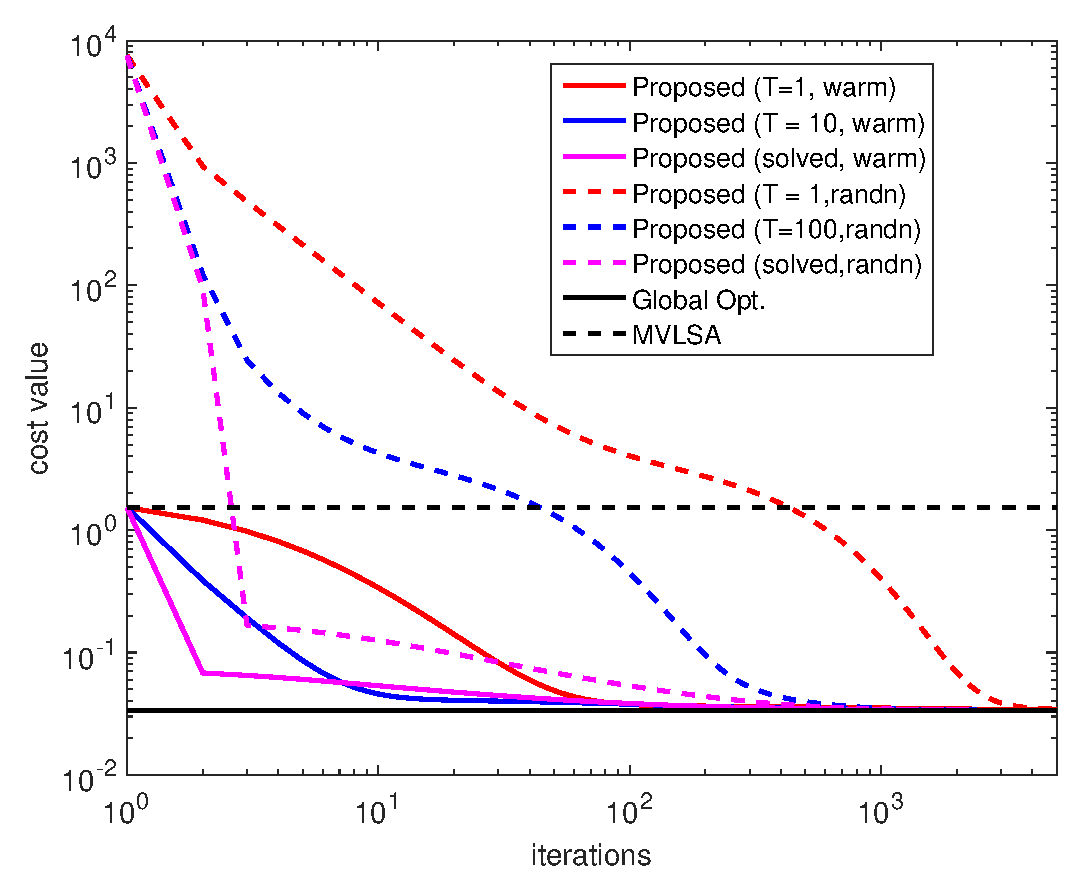
\includegraphics[width=.75\linewidth]{lambda_1.eps} 
\caption{Convergence curves. Small size}
\label{fig:subfigure1}
\end{figure}
In this subsection, we first use small-size problem instances to verify the convergence properties
that were discussed in the last section and also showcase the effectiveness of the algorithm.
\subsubsection{Original Max-Var GCCA}
We generate the synthetic data in the following way: First, we let ${\bm Z}\in\mathbb{R}^{L\times N}$ be a common latent factor of different views,
where the entries of ${\bm Z}$ are drawn from the zero-mean i.i.d. Gaussian distribution and $L\geq N$.
Then, a `mixing matrix' ${\bm A}_i\in\mathbb{R}^{N\times M_i}$ is multiplied to ${\bm Z}$, resulting in ${\bm Y}_i={\bm Z}{\bm A}_i$.
We let $M_1=\ldots=M_I=M$ in this section.
Finally, we add noise so that ${\bm X}_i={\bm Y}_i + \sigma{\bm N}_i$.
Here, ${\bm A}_i$ and ${\bm N}_i$ are generated in the same way as ${\bm Z}$.
We first apply the algorithm with the regularization term $g_i(\cdot)=\mu_i\|\cdot\|_F^2$ and let $\mu_i=0.1$. 
Since $L$ and $M$ are small in this subsection, we employ the optimal solution that is based on eigen-decomposition as a baseline, since this case is solvable.
The multiview latent semantic analysis (\texttt{MVLSA}) algorithm that was proposed in \cite{rastogimultiview} as baselines. 
Recall that \texttt{MVLSA} approximates the views using several leading singular values and vectors.

In Fig.~\ref{fig:subfigure1}, we let $(L,M,N,I)=(500,25,20,3)$. 
We set $\sigma=0.1$ in this case, let $P=8$ and $\gamma=1$ for \texttt{MVLSA} and \texttt{AltMaxVar}, respectively, and ask for $K=5$ canonical components.
The results are averaged over 50 random trials, where ${\bm Z}$, $\{{\bm A}_i\}$, $\{{\bm N}_i\}$ are randomly generated in each trial.
We test the proposed algorithm under different settings:
We let $T=1$, $T=10$, and the gradient descent run until the inner loop converges (denoted as `solved' in the figures).
We also initialize the algorithm with random initializations (denoted as `randn') and warm starts (denoted as `warm') -- i.e., using the solutions of \texttt{MVLSA} as starting points. 
Some observations from Fig.~\ref{fig:subfigure1} are in order. 
First, the proposed algorithm using various $T$'s including $T=1$ and random initialization can reach the global optimum, which supports the analysis in Theorem~\ref{thm:main}.
Second, by increasing $T$, the overall cost value decreases faster in terms of number of outer iterations -- using $T=10$ already gives very good speed of decreasing the cost value.
Third, \texttt{MVLSA} cannot attain the global optimum, as expected. However, it provides good initialization: Using the warm start, the cost value comes close to the optimal value within 100 iterations in this case, even when $T=1$ is employed.
In fact, the combination of \texttt{MVLSA}-based initialization and using $T=1$ offers the most computationally efficient way of implementating the proposed algorithm -- especially for the large-scale case.
In the remaining part of this section, we will employ \texttt{MVLSA} as the initialization of \texttt{AltMaxVar} and perform the $\Q$-subproblem
with $T=1$.



\subsubsection{Feature-Selective Max-Var GCCA}
To test the proposed algorithm with non-smooth regularizers,
we generate cases where outlying features are present in all views.
Specifically, we let ${\bm X}_i=[{\bm Z}{\bm A}_i,{\bm O}_i] + \sigma{\bm N}_i$,
where ${\bm O}_i\in\mathbb{R}^{L\times N_o}$ denotes the irrelevant outlying features and the elements of ${\bm O}_i$ follows the i.i.d. zero-mean unit-variance Gaussian distribution.
We wish the algorithm to perform MAX-VAR GCCA of the views while discounting ${\bm O}_i$ at the same time. 
To deal with outlying features, we employ the regularizer $g_i(\cdot)=\mu_i\|\cdot\|_{2,1}$.
Under such cases, the optimal solution to Problem \eqref{eq:CGCCA_reg} is unknown.
Nevertheless, we evaluate the performance by observing
\begin{align*}
{\rm metric}_1 &=\nicefrac{1}{I}\sum_{i=1}^I\|{\bm X}_i(:,{\cal S}_i^c)\hat{\Q}_i({\cal S}_i^c,:)-\hat{\bm G}\|_F^2,\\
 {\rm metric}_2 &= \nicefrac{1}{I}\sum_{i=1}^I\|{\bm X}_i(:,{\cal S}_i)\hat{\Q}_i({\cal S}_i,:)\|_F^2,
\end{align*}
where ${\cal S}^c_i$ and ${\cal S}_i$ denote the index sets of ``clean'' and outlying features of view $i$, respectively -- i.e., ${\bm X}_i(:,{\cal S}_i^c)={\bm Z}_i{\bm A}_i$ and ${\bm X}_i(:,{\cal S}_i)={\bm O}_i$ if noise is absent.
${\rm metric}_1$ measures the performance of matching $\hat{\bm G}$ with the relevant part of the views, while ${\rm metric}_2$ measures the performance of suppressing the irrelevant part.
We wish an algorithm to give low values of ${\rm metric}_1$ and ${\rm metric}_2$ simultaneously.

Table~\ref{tab:small_sparse} presents the results of a small-size case which are averaged from 50 random trials, where $(L,M,N,I)=(150,60,60,3)$ and $|{\cal S}|=\{61,\ldots,120\}$; i.e.,
$60$ out of $120$ features of $\X_i\in\mathbb{R}^{150\times 120}$ are outlying features.
The average power of the outlying features is set to be the same as that of the clean features, i.e.,
$\|{\bm Q}_i\|_F^2/{\rm nnz}({\bm O}_i)=\|{\bm Z}{\bm A}_i\|_F^2/{\rm nnz}({\bm Z}{\bm A}_i)$ so that the outlying features would have an impact on the CCA result if not discounted.
We ask for $K=10$ canonical components. For \texttt{MVLSA}, we let the rank-truncation parameter to be $P=50$; for \texttt{AltMaxVar}, we set $\gamma=0.99$.
One can see that the eigen-decomposition based algorithm gives similar high values of both the evaluation metrics since it treats $\X_i(:,{\cal S}^c_i)$ and $\X_i(:,{\cal S}_i)$ equally.
It is interesting to see that \texttt{MVLSA} suppresses the irrelevant features to some extent -- although
it does not explicitly consider outlying features, our understanding is that the PCA pre-processing on the views can somewhat suppress the outliers.
Nevertheless, \texttt{MVLSA} does not fit the relevant part of the views well.
The proposed algorithm gives the lowest values of both metrics. In particular, when $\mu=1$, the irrelevant part is almost suppressed completely.
Another observation is that using $\mu=0.5$, the obtained score of ${\rm metric}_1$ is slightly lower than that under $\mu=1$, which makes sense since the algorithm pays more attention to feature selection using a larger $\mu$.
An illustrative example using a random trial can be seen in Fig.~\ref{fig:small_row_norm}.
From there, one can see that the proposed algorithm gives ${\bm Q}_i$'s with almost zero rows over ${\cal S}$, thereby performing feature selection.




% Table generated by Excel2LaTeX from sheet 'simulation'
\begin{table}[htbp]
  \centering
  \caption{Performance of the algorithms when irrelevant features are present. $(L,M,N)=(150,60,60)$; $|{\cal S}|=60$; $\X_i\in\mathbb{R}^{150\times 120}$; $\sigma=1$.}
   	\resizebox{.8\linewidth}{!}{
    \begin{tabular}{c|c|c}
    \hline
    \hline
    Algorithm & ${\rm metric}_1$ &  ${\rm metric}_2$ \\
    \hline
    \hline
    eigen-decomp &9.547&9.547 \\
    \hline
    \texttt{MVLSA} & 15.506	&1.456 \\
    \hline
    proposed ($\mu=.5$) & \textbf{0.486}&	$9.689\times 10^{-3}$ \\
    \hline
    proposed ($\mu=1$) & 1.074 &	${\bf 8.395\times 10^{-4}}$ \\
    \hline
    \hline
    \end{tabular}%
    }
  \label{tab:small_sparse}%
\end{table}%


\begin{figure}[ht]
\centering
{\includegraphics[width=\linewidth]{small_sparse.eps}
\caption{Average row-norms of ${\bm Q}_i$ (i.e., $(1/I)\sum_{i=1}^I\|{\bm Q}_i(m,:)\|_2^2$) for all $m$ given by the algorithms.}
\label{fig:small_row_norm}}
\end{figure}

\subsection{Scalability Test: Large-Size Problems}
%In this subsection, we use large sparse views to test the scalability of the proposed algorithm.

\subsubsection{Original Max-Var GCCA}
We first test the case where no outlying features are involved
and the regularizer $g_i(\cdot)=\mu_i\|\cdot\|_F^2$ is employed.
The views $\X_i={\bm Z}{\bm A}_i+\sigma {\bm N}_i$ are generated following a similar way as in the last subsection, but ${\bm Z}$, ${\bm A}_i$ and ${\bm N}_i$ are sparse so that ${\bm X}_i$ are sparse with a density level $\rho_i$ that is definied as
\[ \rho_i = \frac{{\rm nnz}({\bm X}_i)}{LM}.\]
In the simulations, we let $\rho=\rho_1=\ldots=\rho_I$.
and the results are obtained via averaging 10 random trials.

In Fig.~\ref{fig:runtime_plain}, we show the runtime performance of the algorithms under various sizes of the views.
The density of the views are controlled so that $\rho \leq 10^{-3}$.
We let $M=L\times 0.8$, $M=N$ and change $M$ from $5,000$ to $50,000$.
The eigen-decomposition based global optimal solution and \texttt{MVLSA} (using $P=100$) are used
baselines, and the proposed \texttt{AltMaxVar} is initialized by \texttt{MVLSA} and we let $T=1$.
The diagonal loading parameter is set to be $\mu_i=0.1$ for all algorithms.
One can see that the eigen-decomposition based algorithm does not scale well since the matrix $({\bm X}_i^T{\bm X}_i+\mu_i{\bm I})^{-1}$ is dense.
In particular, the algorithm exhausts the memory quota (32GB RAM) when $M=30,000$. 
\texttt{MVLSA} and the proposed algorithm both scale very well from $M=5,000$ to $M=50,000$:
When $M=20,000$, the global optimal solution uses almost 80 minutes to finish the computations,
while \texttt{MVLSA} and \texttt{AltMaxVar} both use less than 2 minutes.
Note that the runtime of the proposed algorithm already includes the runtime of the initialization time by \texttt{MVLSA}, and thus the runtime curve of \texttt{AltMaxVar} is slightly higher than that of \texttt{MVLSA} in Fig.~\ref{fig:runtime_plain}.
The cost values given by the algorithms can be seen in Table~\ref{tab:cost_large_plain}.
The eigen-decomposition based method gives the lowest cost values when applicable as it is an optimal solution.
In terms of accuracy, the proposed algorithm gives favorable cost values that are close to the optimal value -- note that only one iteration of the ${\bm Q}$-subproblem is implemented.
However, \texttt{MVLSA} is not so promising in terms of cost value.


\begin{figure}[ht]
\centering
{\includegraphics[width=.75\linewidth]{runtime.eps}
\caption{Runtime of the algorithms under various problem sizes. $L=M/0.8$, $\rho\leq 10^{-3}$, $\sigma=0.1$.}
\label{fig:runtime_plain}}
\end{figure}


% Table generated by Excel2LaTeX from sheet 'simulation'
\begin{table}[htbp]
  \centering
   \caption{Cost values of the algorithms under different problem sizes. $L=M/0.8$, $\rho= 10^{-3}$, $\sigma=0.1$. $\dag$ means ``out of memory''.}
    	\resizebox{\linewidth}{!}{\huge
    \begin{tabular}{c|c|c|c|c|c|c}
    \hline
    \hline
    \multirow{2}[4]{*}{Algorithm} & \multicolumn{6}{c}{$M$ } \\
\cline{2-7}          & 5,000  & 10,000 & 20,000 & 30,000 & 40,000 & 50,000 \\
    \hline
    \hline
    Global Opt. & \textbf{0.053 }& \textbf{0.034} &\textbf{ 0.020} & $\dag$ & $\dag$ & $\dag$ \\
    \hline
    \texttt{MVLSA} & 2.103 & 3.749 & 5.135 & 6.018 & 6.579 & 7.044 \\
    \hline
    proposed & 0.088 & 0.062 & 0.047 & 0.043 & 0.041 & 0.039 \\
    \hline
    \hline
    \end{tabular}}%
  \label{tab:cost_large_plain}%
\end{table}%


%\begin{figure}[ht]
%\centering
%{\includegraphics[width=6.15cm]{cost.eps}
%\caption{Cost values given by the algorithms under various problem sizes. $M=L\times 0.8$. For $M\geq 30,000$, the global optimal solution is not provided due to out of memory.}
%\label{fig:cost_plain}}
%\end{figure}

\subsubsection{Feature-Selective Max-Var GCCA}
Table~\ref{tab:rhochange} presents the simulation results of a large-scale case
in the presence of outlying features.
Here, we fix $L=100,000$ and $M=80,000$ and change the density level $\rho$.
We add $|{\cal S}_i|=30,000$ outlying features to each view and every outlying feature is a random sparse vector whose non-zero elements follow the zero-mean i.i.d. unit-variance Gaussian distribution.
We also scale the outlying features as before so that the energy of the clean and outlying features are comparable.
The other settings follow those in the last simulation.
One can see from Table~\ref{tab:rhochange} that the proposed algorithm with $\mu_i=0.5$
gives the most balanced result -- both evaluation metrics are with fairly low levels.
Using $\mu_i=1$ suppresses the $\Q_i({\cal S},:)$ quite well, but using a larger $\mu_i$ also brings some sacrifice to the fitting metric.
In terms of runtime, one can see that the proposed algorithm operates within the same order of magnitude of time as \texttt{MVLSA} does.
Note that the proposed algorithm works with the intact views with the size $L\times M$ but \texttt{MVLSA} works with heavily truncated data.
Therefore, such runtime performance of \texttt{AltMaxVar} is very satisfactory.

Similar results can be seen in Table~\ref{tab:Ichange}, where we let $\rho = 10^{-4}$ and change $I$ from $3$ to $8$. One can see that increasing the number of views does not increase the runtime of the proposed algorithm. The reason is that the updates of different $\Q_i$'s can be easily parallelized.
One can easily implement the parallel computations using the \texttt{parfor} function of \texttt{Matlab} -- which is what we do in this simulation. 

% Table generated by Excel2LaTeX from sheet 'simulation'
\begin{table}[htbp]
  \centering
  \caption{Evaluation of the algorithm under different data densities in the presence of outlying features. $L=100,000$, $M=80,000$, $|{\cal S}|=30,000$, $\sigma=1$, $I=3$.}
   	\resizebox{\linewidth}{!}{\huge 
 \begin{tabular}{c|c|c|c|c|c}
     \hline
     \hline
     \multirow{2}[4]{*}{Algorithm} & \multirow{2}[4]{*}{measure} & \multicolumn{4}{c}{$\rho$ (density of views)} \\
 \cline{3-6}          &       & $10^{-5}$ & $5\times 10^{-4}$ & $10^{-4}$ & $10^{-3}$ \\
     \hline
     \hline
     \multirow{3}[6]{*}{\texttt{MVLSA}} & metric1 & 16.843 & 13.877 & 17.159 & 16.912 \\
 \cline{2-6}          & metric2 & \textbf{0.003} & \textbf{0.010} & 0.009 & 0.003 \\
 \cline{2-6}          & time (min) & \textbf{0.913} & \textbf{1.019} & \textbf{1.252} & \textbf{3.983} \\
     \hline
     \hline
     \multirow{3}[6]{*}{proposed ($\mu=.05$)} & metric1 & \textbf{0.478} & \textbf{0.610} & \textbf{0.565} & \textbf{0.775} \\
 \cline{2-6}          & metric2 & 0.018 & 0.134 & 0.034 & 0.003 \\
 \cline{2-6}          & time  (min) & 3.798	&5.425&	5.765&	24.182 \\
     \hline
     \hline
     \multirow{3}[6]{*}{proposed ($\mu=.1$)} & metric1 & 0.942 & 1.054 & 0.941 & 1.265 \\
 \cline{2-6}          & metric2 & 0.006 & 0.054 & \textbf{0.004} & \textbf{0.000} \\
 \cline{2-6}          & time  (min) & 2.182&	3.791&	4.510&	16.378 \\
     \hline
     \hline
     \multirow{3}[6]{*}{proposed ($\mu=.5$)} & metric1 & 1.592 & 1.497 & 1.306 & 1.538 \\
 \cline{2-6}          & metric2 & \textbf{0.003} & 0.021 & \textbf{0.000} & \textbf{0.000} \\
 \cline{2-6}          & time  (min) & 1.735	&2.714&	3.723	&13.447\\
     \hline
     \hline
     \end{tabular}%
 %
   	}%
  \label{tab:rhochange}%
\end{table}%

% Table generated by Excel2LaTeX from sheet 'simulation'
\begin{table}[htbp]
  \centering
    \caption{Evaluation of the algorithm under different data densities in the presence of outlying features. $L=100,000$, $M=80,000$, $|{\cal S}|=30,000$, $\sigma=1$, $\rho=5\times 10^{-5}$.}
   \resizebox{\linewidth}{!}{\huge     
       \begin{tabular}{c|c|c|c|c|c|c|c}
       \hline
       \hline
       \multirow{2}[4]{*}{Algorithm} & \multirow{2}[4]{*}{measure} & \multicolumn{6}{c}{$I$ (no. of views)} \\
   \cline{3-8}          &       & 3  & 4  & 5 & 6  & 7  & 8 \\
       \hline
       \hline
       \multirow{3}[6]{*}{\texttt{MVLSA}} & metric1 & 15.813 & 15.715 & 14.667 & 16.904 & 17.838 & 17.691 \\
   \cline{2-8}          & metric2 & \textbf{0.008} & 0.009 & 0.009 & 0.009 & 0.007 & 0.009 \\
   \cline{2-8}          & time (min) & \textbf{1.087} & \textbf{0.975} & \textbf{0.960} & \textbf{0.958} & \textbf{0.989} & \textbf{1.026} \\
       \hline
       \hline
       \multirow{3}[6]{*}{proposed ($\mu=.05$)} & metric1 & \textbf{0.731} & \textbf{0.590} & \textbf{0.670} & \textbf{0.611} & \textbf{0.517} & \textbf{0.628} \\
   \cline{2-8}          & metric2 & 0.172 & 0.078 & 0.100 & 0.101 & 0.065 & 0.098 \\
   \cline{2-8}          & time (min) & 5.870&	6.064&	5.762&	5.070&	5.895&	5.776  \\
       \hline
       \hline
       \multirow{3}[6]{*}{proposed ($\mu=.1$)} & metric1 & 1.070 & 1.057 & 1.110 & 1.026 & 1.042 & 1.112 \\
   \cline{2-8}          & metric2 & 0.055 & 0.019 & 0.018 & 0.024 & 0.023 & 0.023 \\
   \cline{2-8}          & time (min) & 3.240&	2.974&	3.313&	3.210&	3.083&	3.529\\
       \hline
       \hline
       \multirow{3}[6]{*}{proposed ($\mu=.5$)} & metric1 & 1.461 & 1.482 & 1.578 & 1.443 & 1.472 & 1.561 \\
   \cline{2-8}          & metric2 & 0.018 & \textbf{0.002} & \textbf{0.003} & \textbf{0.001} & \textbf{0.006} & \textbf{0.007} \\
   \cline{2-8}          & time (min) & 2.700&	2.441&	2.528&	2.569&	2.431&	2.567 \\
       \hline
       \hline
       \end{tabular}%
     \label{tab:addlabel}%
   %
   }%
  \label{tab:Ichange}%
\end{table}%












\subsection{Real-Data Large-Scale Word Embedding Tasks}
We test the algorithms on a large-scale multilingual dataset.
The views are extracted from a large word co-occurrence matrix, which is available at \url{https://sites.google.com/a/umn.edu/huang663/research}.
The original data contains words of three languages, namely, English, Spanish, and French,
and all the words are defined by the co-occurences pointwise mutual information (PMI) with other words.
We use the English words to form our first view, ${\bm X}_1$, which contains $L=183,034$ words and each word is defined by $M_i=100,000$ features (co-occurrences). Note that ${\bm X}_1$ is sparse -- only $1.21\%$ of its entries are non-zeros.
Using a dictionary, we pick out the translations of the English words contained in ${\bm X}_1$ in Spanish and French to form ${\bm X}_2$ and ${\bm X}_3$, respectively.
Note that many English words do not have a corresponding word in Spanish (or French).
In such cases, we simply let ${\bm X}_i(\ell,:)={\bm 0}$ for $i=2$ (or $i=3$),
resulting in sparser ${\bm X}_2$ and ${\bm X}_3$.
Our objective is to find ${\bm G}$ whose rows are the low-dimensional embeddings of the English words (cf. the motivating example in Fig.~\ref{fig:motivation}).

To evaluate the output, we use the evaluation tool provided at {wordvectors.org} \cite{faruqui-2014:SystemDemo}, which runs several word embedding tasks to evaluate a set of given embeddings. Simply speaking, the tasks compare the algorithm-learned
embeddings with the judgment of humans and yield high scores if the embeddings are consistent with the humans. The scores are between zero and one,
and a score equal to one means a perfect alignment between the learned result and human judgment.
We use the result of \texttt{MVLSA} with $P=640$ as benchmark. 
The result of applying SVD to ${\bm X}_1$ without considering different languages is also presented.
We apply the proposed algorithm warm started by \texttt{MVLSA} and set $T=1$.
We run two versions of our algorithm. The first one uses $g_i(\cdot)=\|\cdot\|_F^2$
for $i=1,2,3$.
The second one uses $g_i(\cdot)=0.05\|\cdot\|_{2,1}$ for $i=2,3$.
The reason for adding $\ell_2/\ell_1$ mixed norm regularization to the French and Spanish views
is towfold:
First, the $\ell_2/\ell_1$ norm promotes row sparsity of $\Q_i$ and thus performs feature selection on $\X_2$ and $\X_3$ -- this physically means that we aim at selecting the most useful features from the other languages to help enhance English word embeddings.
Second, the languages are effectively `fat matrices' and thus need to use a column-selective regularizer can help improve the conditioning.


Tables~\ref{tab:K50} and \ref{tab:K100} show the word embedding results using $K=50$ and $K=100$, respectively.
We see that using the information from multiviews does help in improving the word embeddings:
For $K=50$ and $K=100$, the multiview approaches perform better relative to SVD in 11 and 8 tasks out of 12 tasks. 
In addition, the proposed algorithm with the regularizer $g_i(\cdot)=\|\cdot\|_F^2$ gives similar or slightly better in average on both experiments compared to \texttt{MVLSA}.
The proposed algorithm with the feature-selective regularizer ($g_i(\cdot)=\mu_i\|\cdot\|_{2,1}$) gives the best evaluation results on both experiments -- this suggests that for large-scale multiview analysis, feature selection is much meaningful.


% Table generated by Excel2LaTeX from sheet 'Sheet1'
% Table generated by Excel2LaTeX from sheet 'Sheet1'
\begin{table}[htbp]
  \centering
  \caption{Evaluation on 12 word embedding tasks; $K=50$.}
  	\resizebox{\linewidth}{!}{\huge
        \begin{tabular}{c|c|c|c|c}
        \hline
        \hline
        \multirow{2}[4]{*}{Task} & \multicolumn{4}{c}{Algorithm ($K=50$)}\\
    \cline{2-5}          & SVD   & \texttt{MVLSA} & Proposed ($\|\cdot\|_F^2$) & Proposed  ($\|\cdot\|_{2,1}$)\\
        \hline
        \hline
        EN-WS-353-SIM & 0.63  & \textbf{0.69} & 0.67  & 0.68\\
        \hline
        EN-MC-30 & 0.56  & 0.63  & 0.63  & \textbf{0.64}\\
        \hline
        EN-MTurk-771 & 0.54  & 0.58  & 0.59  & \textbf{0.60}\\
        \hline
        EN-MEN-TR-3k & 0.67  & 0.66  & 0.67  & \textbf{0.68}\\
        \hline
        EN-RG-65 & 0.51  & 0.53  & 0.55  & \textbf{0.58}\\
        \hline
        EN-MTurk-287 & \textbf{0.65} & 0.64  & \textbf{0.65} & 0.64\\
        \hline
        EN-WS-353-REL & 0.50  & 0.51  & 0.53  & \textbf{0.55}\\
        \hline
        EN-VERB-143 & 0.21  & \textbf{0.22} & 0.21  & 0.21\\
        \hline
        EN-YP-130 & 0.36  & 0.39  & 0.38  & \textbf{0.41}\\
        \hline
        EN-SIMLEX-999 & 0.31  & \textbf{0.42} & 0.41  & 0.39\\
        \hline
        EN-RW-STANFORD & 0.39  & \textbf{0.43} & \textbf{0.43} & \textbf{0.43}\\
        \hline
        EN-WS-353-ALL & 0.56  & 0.59  & 0.59  & \textbf{0.60}\\
        \hline
        \hline
        Average & 0.49  & 0.52  & 0.53  & \textbf{0.54}\\
        \hline
        Median & 0.53  & 0.56  & 0.57  & \textbf{0.59}\\
        \hline
        \hline
        \end{tabular}%
    
    }%
  \label{tab:K50}%
\end{table}%

% Table generated by Excel2LaTeX from sheet 'July31'
\begin{table}[htbp]
  \centering
  \caption{Evaluation on 12 word embedding tasks; $K=100$.}  
  	\resizebox{\linewidth}{!}{\huge
    \begin{tabular}{c|c|c|c|c}
    \hline
    \hline
    \multirow{2}[4]{*}{Task} & \multicolumn{4}{c}{Algorithm ($K=100$)}\\
\cline{2-5}          & SVD   & \texttt{MVLSA} & Proposed ($\|\cdot\|_F^2$) & Proposed  ($\|\cdot\|_{2,1}$)\\
    \hline
    \hline
    EN-WS-353-SIM & 0.68  & \textbf{0.72} & 0.71  & \textbf{0.72}\\
    \hline
    EN-MC-30 & 0.73  & 0.68  & 0.72  & \textbf{0.74}\\
    \hline
    EN-MTurk-771 & 0.59  & 0.60  & 0.60  & \textbf{0.61}\\
    \hline
    EN-MEN-TR-3k & \textbf{0.72} & 0.70  & 0.70  & 0.71\\
    \hline
    EN-RG-65 & \textbf{0.68} & 0.63  & 0.64  & \textbf{0.68}\\
    \hline
    EN-MTurk-287 & 0.61  & \textbf{0.66} & 0.65  & 0.64\\
    \hline
    EN-WS-353-REL & \textbf{0.57} & 0.54  & 0.55  & 0.56\\
    \hline
    EN-VERB-143 & 0.19  & 0.28  & 0.27  & \textbf{0.29}\\
    \hline
    EN-YP-130 & 0.42  & 0.41  & 0.41  & \textbf{0.45}\\
    \hline
    EN-SIMLEX-999 & 0.34  & \textbf{0.42} & 0.41  & 0.41\\
    \hline
    EN-RW-STANFORD & 0.44  & \textbf{0.46} & 0.45  & \textbf{0.46}\\
    \hline
    EN-WS-353-ALL & \textbf{0.62} & \textbf{0.62} & \textbf{0.62} & \textbf{0.62}\\
    \hline
    \hline
    Average & 0.55  & 0.56  & 0.56  & \textbf{0.58}\\
    \hline
    Median & 0.60  & 0.61  & 0.61  & \textbf{0.62}\\
    \hline
    \hline
    \end{tabular}%
    }
  \label{tab:K100}%
\end{table}%


\section{Conclusion}
In this work, we revisited the MAX-VAR GCCA problem with an eye towards scenarios involving large-scale and sparse data. 
The proposed approach is memory-efficient and has light per-iteration computational complexity if the views are sparse, and is thus suitable for dealing with big data.
The algorithm is also flexible for incorporating different structure-promoting regularizers on the canonical components such as the feature-selective regularizations.
A thorough convergence analysis was presented, showing that the proposed algorithmic framework
guarantees a KKT point to be obtained with a sublinear rate in general cases with a variety of structure-promoting regularizers.
We also showed that the algorithm guarantees approaching a global optimal solution with a linear convergence rate if the original MAX-VAR problem is considered.
Simulations and careful experiments with large-scale multi-lingual data showed that the performance of the proposed algorithm is promising in dealing with large and sparse multiview data.



\ifplainver
    \section*{Appendix}
    \renewcommand{\thesubsection}{\Alph{subsection}}
\else
\appendices
\fi



\section{Proof of Proposition~\ref{lem:monotonicity}}
Recall that we have defined ${\bm Q}=[{\bm Q}_1^T,\ldots,{\bm Q}_I^T]^T$ as a collection 
of $\Q_i$'s
and we define
$F({\bm G},{\bm Q}) = \sum_{i=1}^{I}\frac{1}{2}\left\|{\bm X}_i{\bm Q}_i-{\bm G}\right\|_F^2 + \sum_{i=1}^Ig_i(\Q_i)$.
Since the algorithm is essentially a two-block alternating optimization (i.e., ${\bm Q}_i$ for all $i$ are updated simultaneously), the above notation suffices to describe the updates.
We also define
\begin{align*}
u_Q\left(\Q;\hat{\bm G},\hat{\bm Q}\right) = &f(\hat{\bm G},\hat{\bm Q}) +  \left<\nabla_{{\bm Q}} f(\hat{\bm Q},\hat{\bm G}),{\bm Q}-\hat{\bm Q}\right>\\
&+ \sum_{i=1}^I\frac{1}{2\alpha_i}\|{\bm Q}_i-\hat{\bm Q}\|_F^2+ \sum_{i=1}^Ig_i(\Q_i);
\end{align*}
i.e., $u_Q\left({\bm Q};\hat{\bm G},\hat{\bm Q}\right)$ is an approximation of $F({\bm G},{\bm Q})$
locally at the point $(\hat{\bm G},\hat{\bm Q})$.
We further define
%\begin{equation*}
%\begin{aligned}
$\tilde{u}_Q\left(\Q;\hat{\bm G},\hat{\bm Q}\right) = u_Q\left({\bm Q};\hat{\bm G},\hat{\bm Q}\right) -\sum_{i=1}^Ig_i(\Q_i)$;
%\end{aligned}
%\end{equation*}
i.e., $\tilde{u}_Q\left(\Q;\hat{\bm G},\hat{\bm Q}\right)$ is an approximation of the continuously differentiable part $f({\bm G},{\bm Q})$
locally at the point $(\hat{\bm G},\hat{\bm Q})$.
One can see that,
\begin{subequations}\label{eq:gradequal}
\begin{align}
	&\nabla_{{\bm Q}_i} f\left(\hat{\bm G},\hat{\bm Q}\right)=\nabla_{{\bm Q}} \tilde{u}\left(\hat{\bm Q};\hat{\bm G},\hat{\bm Q}\right),\\
	& \nabla_{{\bm Q}} f\left(\hat{\bm G},\hat{\bm Q}\right) + \partial_{\Q} g(\hat{\Q}) = \nabla_{{\bm Q}}\tilde{u}\left(\hat{\bm Q};\hat{\bm G},\hat{\bm Q}\right) + \partial_{\Q} g(\hat{\Q}).
\end{align}
\end{subequations}
Since $\nabla_{{\bm Q}_i} f({\bm G},{\bm Q})$ is $L_i$-Lipschitz continuous w.r.t. ${\bm Q}_i$ and $\alpha_i\leq 1/L_i$ for all $i$, we have the following holds:
\begin{equation}\label{eq:gleqf}
	u_Q\left({\bm Q};\hat{\bm G},\hat{\bm Q}\right)\geq F\left(\hat{\bm G},{\bm Q}\right),~\forall~{\bm Q},
\end{equation}
where the equality holds if and only if ${\bm Q}_i = \hat{\bm Q}_i$ for all $i$, i.e.,
\begin{equation}\label{eq:geqf}
u_Q\left(\hat{\bm Q};\hat{\bm G},\hat{\bm Q}\right) = F\left(\hat{\bm G},\hat{\bm Q}\right).
\end{equation}
Now, let us denote by ${\bm Q}^{(r,t)}$ (where $0\leq t\leq T-1$) the solution of ${\bm Q}$
after $t$ PG updates when ${\bm G}^{(r)}$ is fixed, where $r$ is the iteration index of the outer loop.
With the above notation, we have ${\bm Q}^{(r,0)}={\bm Q}^{(r)}$ and ${\bm Q}^{(r,T)}={\bm Q}^{(r+1)}$.
Also, it can be seen that the update of ${\bm Q}_i$ can be written as \cite{beck2009fast}:
\begin{equation}\label{eq:updateQ}
\begin{aligned}
	{\bm Q}_i^{(r,t+1)}= \arg\min_{{\bm Q}_i}~u_{Q}\left( {\bm Q};{\bm G}^{(r)},{\bm Q}^{(r,t)} \right).
\end{aligned}
\end{equation}


Similarly, we define
\begin{align*}
u_G\left(\G;\hat{\bm G},\hat{\bm Q}\right) = &f(\hat{\bm G},\hat{\bm Q}) + \left<\nabla_{\G} f(\hat{\bm G},\hat{\bm Q}),\G-\hat{\bm G}\right>\\
& + \frac{I}{2\gamma}\left\|\G-\hat{\G}\right\|_F^2+ \sum_{i=1}^Ig_i(\hat{\Q_i}),
\end{align*}
where the last term is a constant if $\Q$ is fixed.
We also have the following holds:
\begin{equation}\label{eq:Ggradequal}
\begin{aligned}
	&\nabla_{\G} f\left(\hat{\bm G},\hat{\bm Q}\right)=\nabla_{\G} {u}\left(\hat{\bm G};\hat{\bm G},\hat{\bm Q}\right)=I\cdot\hat{\bm G} - \sum_{i=1}^I{\X_i\Q_i}.
\end{aligned}
\end{equation}

The update rule of $\G$ in Algorithm~\ref{algo:AltCCA} can be re-expressed as follows:
\begin{align*}
 \G \in & \arg\min_{\G^T\G={\bm I}}~\left\|\G - \left((1-\gamma)\hat{\G}+\gamma \sum_{i=1}^I\nicefrac{\X_i\Q_i}{I}\right)\right\|_F^2 \\
\Leftrightarrow  \G  \in & \arg\min_{\G^T\G={\bm I}}~\left\|\G - \left(\hat{\G}-(\nicefrac{\gamma}{I}) \nabla_{\G} f\left(\hat{\bm G},\hat{\bm Q}\right)\right)\right\|_F^2\\
\Leftrightarrow   \G  \in & \arg\min_{\G^T\G={\bm I}}~u_G\left(\G;\hat{\bm G},\hat{\bm Q}\right)
\end{align*}
Since $\nabla_{\G} f({\bm G},{\bm Q})$ is $I$-Lipschitz continuous w.r.t. $\G$ and $\gamma\leq 1$, we have
\begin{equation}\label{eq:ugleqf}
	u_G\left({\bm G};\hat{\bm G},\hat{\bm Q}\right)\geq F\left({\bm G},\hat{\bm Q}\right),~
	u_G\left(\hat{\bm G};\hat{\bm G},\hat{\bm Q}\right)= F\left(\hat{\bm G},\hat{\bm Q}\right).
\end{equation}
Hence, Algorithm~\ref{algo:AltCCA} boils down to
\begin{subequations}
\begin{align}
{\bm Q}_i^{(r,t+1)}&= \arg\min_{{\bm Q}_i}~u_{Q}\left( {\bm Q};{\bm G}^{(r)},{\bm Q}^{(r,t)} \right),\quad \forall t\label{eq:q_update_u}\\
\G^{(r+1)} &\in \arg\min_{\G^T\G={\bm I}}~u_G\left(\G;{\bm G}^{(r)},{\bm Q}^{(r+1)}\right). \label{eq:g_update_u}
\end{align}
\end{subequations}
When $\gamma=1$, \eqref{eq:g_update_u} amounts to SVD of $\sum_{i=1}^I\X_i\Q_i/I$ and the ${\bm G}$-subproblem $\min_{\G^T\G={\bm I}}F({\bm Q}^{(r+1)},\G)$ is optimally solved;
otherwise, both \eqref{eq:q_update_u} and \eqref{eq:g_update_u} are local upper bound minimizations.



Note that the following holds:
%\begin{subequations}\label{eq:mono}
%\begin{align}
%        & F\left({\bm G}^{(r)},{\bm Q}^{(r)}\right)  = u_Q(\Q^{(r)};{\bm G}^{(r)},{\bm Q}^{(r)}) \label{eq:mono1}\\
%         & \geq u_Q(\Q^{(r,1)};{\bm G}^{(r)},{\bm Q}^{(r,0)}) \geq F\left({\bm G}^{(r)},{\bm Q}^{(r,1)}\right) \label{eq:mono12}\\
%         & = u_Q(\Q^{(r,1)};{\bm G}^{(r)},{\bm Q}^{(r,1)}) \geq u_Q(\Q^{(r,2)};{\bm G}^{(r)},{\bm Q}^{(r,1)}) \label{eq:mono14}\\
%         &\vdots\\
%%                                                   & \geq u_Q(\Q^{(r,t)};{\bm G}^{(r)},{\bm Q}^{(r,t-1)}) \label{eq:mono2}\\
%         & \geq u_Q(\Q^{(r+1)};{\bm G}^{(r)},{\bm Q}^{(r,T-1)}) \geq F\left({\bm G}^{(r)},{\bm Q}^{(r+1)}\right) \label{eq:mono4}\\
%                                                   &= u_G\left({\bm G}^{(r)};{\bm G}^{(r)},{\bm Q}^{(r+1)}\right) \label{eq:mono5}\\
%												   &\geq u_G\left({\bm G}^{(r+1)};{\bm G}^{(r)},{\bm Q}^{(r+1)}\right) \label{eq:mono6}\\
%												   &\geq F\left({\bm G}^{(r+1)},{\bm Q}^{(r+1)}\right), \label{eq:mono7}
%\end{align}
%\end{subequations}
\begin{subequations}\label{eq:mono}
\begin{align}
         F\left({\bm G}^{(r)},{\bm Q}^{(r)}\right) & = u_Q(\Q^{(r)};{\bm G}^{(r)},{\bm Q}^{(r)}) \label{eq:mono1}\\
%                                                   & \geq u_Q(\Q^{(r,1)};{\bm G}^{(r)},{\bm Q}^{(r,0)}) \label{eq:mono11}\\
%                                                   & \geq F\left({\bm G}^{(r)},{\bm Q}^{(r,1)}\right) \label{eq:mono12}\\
%                                                   & = u_Q(\Q^{(r,1)};{\bm G}^{(r)},{\bm Q}^{(r,1)}) \label{eq:mono13}\\
%                                                   & \geq u_Q(\Q^{(r,2)};{\bm G}^{(r)},{\bm Q}^{(r,1)}) \label{eq:mono14}\\
%                                                   &\vdots\\
%                                                   & \geq u_Q(\Q^{(r,t)};{\bm G}^{(r)},{\bm Q}^{(r,t-1)}) \label{eq:mono2}\\
                                                   & \geq u_Q(\Q^{(r+1)};{\bm G}^{(r)},{\bm Q}^{(r,T-1)}) \label{eq:mono3}\\
                                                   &\geq F\left({\bm G}^{(r)},{\bm Q}^{(r+1)}\right) \label{eq:mono4}\\
                                                   &= u_G\left({\bm G}^{(r)};{\bm G}^{(r)},{\bm Q}^{(r+1)}\right) \label{eq:mono5}\\
												   &\geq u_G\left({\bm G}^{(r+1)};{\bm G}^{(r)},{\bm Q}^{(r+1)}\right) \label{eq:mono6}\\
												   &\geq F\left({\bm G}^{(r+1)},{\bm Q}^{(r+1)}\right), \label{eq:mono7}
\end{align}
\end{subequations}
where \eqref{eq:mono1} holds because of \eqref{eq:geqf}, \eqref{eq:mono3} holds
since PG is a descending method when $\alpha_i\leq 1/L_i$ \cite{beck2009fast},
\eqref{eq:mono4} holds by the property in \eqref{eq:geqf},
\eqref{eq:mono5} holds due to \eqref{eq:ugleqf},
\eqref{eq:mono6} is due to the fact that \eqref{eq:g_update_u} is optimally solved,
and \eqref{eq:mono7} holds also because of the first equation in \eqref{eq:ugleqf}.

Next, we show that every limit point is a KKT point.
Assume that there exists a convergent subsequence of $\{{\bm G}^{(r)},{\bm Q}^{(r)}\}_{r=0,1,\ldots}$,
whose limit point is $({\bm G}^\ast,{\bm Q}^\ast)$ and the subsequence is indexed by $\{r_j\}_{j=1,\ldots,\infty}$.
We have the following chain of inequalities:
\begin{subequations}\label{eq:u_Q}
\begin{align}
         u_Q\left({\bm Q};{\bm G}^{(r_j)},{\bm Q}^{(r_j)}\right) &\geq u_Q\left({\bm Q}^{(r_j,1)};{\bm G}^{(r_j)},{\bm Q}^{(r_j)}\right) \label{eq:cmin1}\\
%				                               &\geq f\left({\bm G}^{(r_j)},{\bm Q}^{(r_j,1)}\right)  \label{eq:cmin2}\\
%				                               & =  g\left({\bm Q}^{(r_j,1)};{\bm G}^{(r_j)},{\bm Q}^{(r_j,1)}\right) \label{eq:cmin21}\\
%				                               &\geq g\left({\bm Q}^{(r_j,2)};{\bm G}^{(r_j)},{\bm Q}^{(r_j,1)}\right) \label{eq:cmin22}\\
%				                               &\vdots \nonumber\\
				                               &\geq u_Q\left({\bm Q}^{(r_j,T)};{\bm G}^{(r_j)},{\bm Q}^{(r_j,T-1)}\right) \label{eq:cmin23}\\
				                              &\geq F({\bm G}^{(r_j)},{\bm Q}^{(r_j+1)})\label{eq:cmin24}\\					
                                               &\geq F\left({\bm G}^{(r_j+1)},{\bm Q}^{(r_j+1)}\right)  \label{eq:cmin3}\\
											  &\geq F\left({\bm G}^{(r_{j+1})},{\bm Q}^{(r_{j+1})}\right)  \label{eq:cmin4}\\
											   & = u_Q\left({\bm Q}^{(r_{j+1})};{\bm G}^{(r_{j+1})},{\bm Q}^{(r_{j+1})}\right), \label{eq:cmin5}
\end{align}
\end{subequations}
where \eqref{eq:cmin1} holds because of the update rule in \eqref{eq:q_update_u},
\eqref{eq:cmin23} holds, again, by the descending property of PG,
\eqref{eq:cmin3} follows \eqref{eq:mono7},
and \eqref{eq:cmin5} is again because of the way that we construct $u_Q({\bm Q};{\bm G}^{(r_{j+1)}},{\bm Q}^{(r_{j+1})})$.
Taking $j\rightarrow \infty$, and by continuity of $u_Q(\cdot)$, we have
\begin{equation}
	    u_Q({\bm Q};{\bm G}^{\ast},{\bm Q}^\ast) \geq  u_Q({\bm Q}^\ast;{\bm G}^{\ast},{\bm Q}^\ast),
\end{equation}
i.e., ${\bm Q}^{\ast}$ is a minimum of $u_Q({\bm Q};{\bm G}^{\ast},{\bm Q}^\ast)$.
Consequently, ${\bm Q}^{\ast}$ satisfies the conditional KKT conditions, i.e.,
%\begin{equation*}
$	 {\bm 0} \in  \nabla_{{\bm Q}} \tilde{u}_Q({\bm Q}^\ast;{\bm G}^{\ast},{\bm Q}^\ast) + \partial_{\Q}g(\Q^\ast),$
%\end{equation*}
which also means that the following holds:
\begin{equation}\label{eq:QKKT}
	     {\bm 0} \in \nabla_{{\bm Q}_i} f({\bm G}^{\ast},{\bm Q}^\ast) + \partial_{\Q}g(\Q^\ast) ,
\end{equation}
following \eqref{eq:gradequal}.

We now show that $\Q^{(r_j,t)}$ for $t=1,\ldots,T$ also converges to $\Q^\ast$.
Indeed, we have
\begin{align*}
u_Q(\Q^{(r_{j+1})};\G^{(r_{j+1})},\Q^{(r_{j+1})})&\leq u_Q(\Q^{(r_j,1)};\G^{(r_j)},\Q^{(r_j)})\\
&\leq u_Q(\Q^{(r_j)};\G^{(r_j)},\Q^{(r_j)}) ,
\end{align*}
where the first inequality was derived from \eqref{eq:u_Q}.
Taking $j\rightarrow \infty$, we see that
$ u_Q(\Q^{\ast};\G^{\ast},\Q^{\ast})\leq u_Q(\Q^{(r_j,1)};\G^{\ast},\Q^{\ast})\leq u_Q(\Q^{\ast};\G^{\ast},\Q^{\ast}) , $
which implies that
$u_Q(\Q^{(r_j,1)};\G^{\ast},\Q^{\ast})= u_Q(\Q^{\ast};\G^{\ast},\Q^{\ast})\leq u_Q(\Q;\G^{\ast},\Q^{\ast}).$
On the other hand, the problem in \eqref{eq:q_update_u} has a unique minimizer when $g_i(\cdot)$ is a convex closed function \cite{parikh2013proximal},
which means that $\Q^{(r_j,1)}\rightarrow \Q^{\ast}$. By the same argument, we can show that
$\Q^{(r_j,t)}$ for $t=1,\ldots,T-1$ also converges to $\Q^\ast$ using the same argument.
Consequently, we have
$\Q^{(r_j,T)} = \Q^{(r_j+1)} \rightarrow \Q^\ast$. 
Now, we repeat the proof in \eqref{eq:u_Q} to ${\bm G}$:
\begin{subequations}\label{eq:u_G}
\begin{align*}
         u_G\left({\bm G};{\bm G}^{(r_j)},{\bm Q}^{(r_j+1)}\right) &\geq u_G\left({\bm G}^{(r_j+1)};{\bm G}^{(r_j)},{\bm Q}^{(r_j+1)}\right) \\
				                              &\geq F({\bm G}^{(r_j+1)},{\bm Q}^{(r_j+1)})\\					
                                               &\geq F\left({\bm G}^{(r_j+1)},{\bm Q}^{(r_j+1)}\right)  \\
%											  &\geq F\left({\bm G}^{(r_{j+1})},{\bm Q}^{(r_{j+1})}\right)  \\
											   & = u_G\left({\bm G}^{(r_{j+1})};{\bm G}^{(r_{j+1})},{\bm Q}^{(r_{j+1})}\right), 
\end{align*}
\end{subequations}
Taking $j\rightarrow \infty$ and by $\Q^{(r_j+1)} \rightarrow \Q^\ast$, we have
\[ u_G\left({\bm G};{\bm G}^{\ast},{\bm Q}^{\ast}\right) \geq u_G\left({\bm G}^{\ast};{\bm G}^{\ast},{\bm Q}^{\ast}\right),\quad \forall \G^T\G={\bm I}. \]
The above means that $\G^\ast$ satisfies the partial conditional KKT conditions w.r.t. $\G$.
%\begin{equation}\label{eq:GKKT}
%	   \begin{cases}
%	  \nabla_{{\bm G}} f({\bm G}^{\ast},{\bm Q}^\ast) - {\bm G}^\ast{\bm \Lambda}^\ast = {\bm 0},\\
%	  (\G^\ast)^T\G^\ast = {\bm I},
%	   \end{cases}
%\end{equation}
%where ${\bm \Lambda}$ is a dual variable associated with the constraint ${\bm G}^T{\bm G}={\bm I}$, and is symmetric \cite{wen2013feasible}.
Combining with \eqref{eq:QKKT}, we see that $({\bm G}^\ast,{\bm Q}^\ast)$ is a KKT point of the original problem. 

\bigskip

Now, we show the b) part.
First, we show that ${\bm Q}_i$ remains in a bounded set (the variable ${\bm G}$ is always bounded since we keep it feasible in each iteration). 
Since the objective value is non-increasing (cf. Proposition~\ref{lem:monotonicity}), if we denote the initial objective value as $V$, then $F({\bm G}^{(r)},{\bm Q}^{(r)}) \leq V$ holds in all subsequent iterations.  
Note that when ${\bm X}_i^{(0)}$ and ${\bm Q}_i^{(0)}$ are bounded, $V$ is also finite. 
In particular, we have $\left\| {\bm X}_i {\bm Q}_i - {\bm G} \right\|_F^2 + 2\sum_{i=1}^Ig_i(\Q_i) \leq 2V$
holds, which implies
$ \| {\bm X}_i {\bm Q}_i \|_F \leq \| {\bm G} \|_F + \sqrt{2V}$
by the triangle inequality.
The right-hand side is finite since both terms are bounded. Denote $ ( \| {\bm G} \|_F + \sqrt{2V} )$ by $V'$. Then, we have
$\| {\bm Q}_i \|_F = \| ({\bm X}_i^T{\bm X}_i)^{-1} {\bm X}_i^T{\bm X}_i {\bm Q}_i \|_F
\leq \| ({\bm X}_i^T{\bm X}_i)^{-1} {\bm X}_i^T \|_F \cdot \|{\bm X}_i {\bm Q}_i \|_F
\leq V' \cdot \| ({\bm X}_i^T{\bm X}_i)^{-1} {\bm X}_i^T \|_F.$
%\begin{align*}
%\| {\bm Q}_i \|_F &= \| ({\bm X}_i^T{\bm X}_i)^{-1} {\bm X}_i^T{\bm X}_i {\bm Q}_i \|_F\\
%&\leq \| ({\bm X}_i^T{\bm X}_i)^{-1} {\bm X}_i^T \|_F \cdot \|{\bm X}_i {\bm Q}_i \|_F\\
%&\leq V' \cdot \| ({\bm X}_i^T{\bm X}_i)^{-1} {\bm X}_i^T \|_F.
%\end{align*} 
Now, by the assumption that ${\rm rank}({\bm X}_i)=M_i$, the term $\| ({\bm X}_i^T{\bm X}_i)^{-1} {\bm X}_i^T \|_F$ is bounded.  This shows that $\| {\bm Q}_i \|_F$ is bounded.
Hence, starting from a bounded ${\bm Q}_i^{(0)}$, the solution sequence $\{{\bm Q}{(r)},{\bm G}^{(r)}\}$ remains in a bounded set. Since the constraints of ${\bm Q}_i$, i.e., $\mathbb{R}^{M_i\times K}$ and ${\bm G}$ are also closed sets,  $\{{\bm Q}^{(r)},{\bm G}^{(r)}\}$ remains in a compact set.

Now, let us denote ${\cal K}$ as the set containing all the KKT points.
Suppose the whole sequence does not converge to ${\cal K}$.
Then, there exists a convergent subsequence indexed by $\{r_j\}$ such that
$\lim_{j\rightarrow \infty} d^{(r)}({\cal K})\geq \gamma$
for some positive $\gamma$, where
$d^{(r)}({\cal K}) = \min_{{\bm Y}\in{\cal K}}~\|({\bm G}^{(r)},{\bm Q}^{(r)}) - {\bm Y}\|.$
Since the subsequence indexed by $\{r_j\}$ lies in a closed and bounded set as we have shown,
this subsequence has a limit point.
However, as we have shown in Theorem~\ref{lem:monotonicity}, every limit point of the solution sequence is a KKT point.
This is a contradiction.
Therefore, the whole sequence converges to a KKT point.
%\hfill $\square$

\section{Proof of Lemma~\ref{lem:z}}\label{app:lemma_z}
First, we have the update rule
$\Q_i^{(r,t+1)} = \Q_i^{(r,t)}-\alpha_i\tilde{\nabla}_{\Q_i}F(\Q_i^{(r,t)},\G^{(r)}),$
which yields the following relationship:
\begin{equation}\label{eq:q_norm}
\frac{1}{\alpha_i}(\Q_i^{(r,t+1)} - \Q_i^{(r,t)} )= -\tilde{\nabla}_{\Q_i}F(\Q_i^{(r,t)},\G^{(r)}).
\end{equation}
Meanwhile, the updating rule can also be expressed as
\begin{align}
\Q_i^{(r+1,t)} = &\arg\min_{\Q_i}~ \left<\nabla_{\Q_i}f(\Q_i^{(r,t)},\G^{(r)}),\Q_i -\Q_i^{(r,t)}\right> \nonumber\\
     & +g_i(\Q_i)+\frac{1}{2\alpha_i}\|\Q_i-\Q_i^{(r,t)}\|_F^2.  \label{eq:q_arg}
\end{align}
Therefore, 
there exists a $\partial_{\Q_i}g_i(\Q^{(r+1,t)})$ and a $\Q^{(r+1,t)}$ satisfy the following optimality conditions:
\begin{align*}
&{\bm 0} = \nabla_{\Q}f(\Q^{(r,t)},\G^{(r)}) + \partial_{\Q}g(\Q^{(r,t+1)})+\frac{1}{\alpha_i}(\Q_i^{(r,t+1)}-\Q_i^{(r,t)}).
\end{align*}
Consequently, we see that
\begin{align*}
&\sum_{i=1}^I\sum_{t=0}^T\left\|\tilde{\nabla}_{\Q_i}F(\Q_i^{(r,t)},\G^{(r)})\right\|_F^2\rightarrow 0 \\
&\Rightarrow \Q_i^{(r,t)}-\Q_i^{(r,t+1)} \rightarrow {\bm 0},~\forall~t=0,\ldots,T-1\\
&\Rightarrow \Q_i^{(r)}-\Q_i^{(r+1)} \rightarrow 0,~\forall i\\
&\Rightarrow \nabla_{\Q}~f\left(\Q^{(r)},\G^{(r)}\right) + \partial_{\Q} g\left(\Q^{(r)}\right)  \rightarrow 0 \nonumber
\end{align*}
which holds since $T$ is finite.
The above means that 
${\bm 0}\in \nabla_{\Q}f(\Q^{(r)},\G^{(r)}) + \partial_{\Q}g(\Q^{(r)})$
is satisfied when $Z^{r,r+1}\rightarrow 0$.


%To keep the notations simple, we prove the theorem using the $T=1$ case.
%The proof of the $T\geq 2$ can be obtained in a straightforward manner. 
%We first show that $Z^{(r,r+1)}\rightarrow 0$ implies that a KKT point is reached.
%First, by the updating rule, we have
%\begin{equation}\label{eq:q_arg}
%\Q^{(r+1)} = \arg\min_{\Q}~ \left<\nabla_{\Q}f(\Q^{(r)},\G^{(r)}),\Q -\Q^{(r)}\right> + r(\Q)+\sum_{i=1}^I\frac{1}{2\alpha_i}\|\Q_i-\Q_i^{(r)}\|_F^2. 
%\end{equation}
%Therefore, $\Q^{(r+1)}$ satisfies the optimality condition of the RHS, i.e.,
%\begin{align}
%&{\bm 0}\in \nabla_{\Q}f(\Q^{(r)},\G^{(r)}) + \partial_{\Q}r(\Q^{(r+1)})+{\bm D}(\Q^{(r+1)}-\Q^{(r)}) \nonumber \\
%\Rightarrow & \|\nabla_{\Q}f(\Q^{(r)},\G^{(r)}) + \partial_{\Q}r(\Q^{(r+1)}) \|_F^2 = \sum_{i=1}^I\frac{1}{\alpha_i^2}\left\|\Q_i^{(r+1)}-\Q_i^{(r)}\right\|_F^2, \label{eq:q_norm}
%\end{align}
%where
%\[{\bm D}={\rm Diag}\left(\frac{1}{\alpha_1}{\bm 1}^T_{M_1},\ldots,\frac{1}{\alpha_I}{\bm 1}^T_{M_I}\right).\]
%The above implies that
%\begin{align}
%\|\nabla_{\Q}f(\Q^{(r)},\G^{(r)}) + \partial_{\Q}r(\Q^{(r+1)}) \|_F^2 \rightarrow 0 \nonumber\\
%\Rightarrow \left\|\Q_i^{(r+1)}-\Q_i^{(r)}\right\|_F^2 \rightarrow 0.
%\end{align}

Recall that the update rule of $\G$ is equivalent to solving
\begin{equation}\label{eq:G_projgrad}
\begin{aligned}
\min_{\G^T\G=\bm I}\quad \left\|\G - \left(\G^{(r)} -\nicefrac{\gamma}{I} \left(\nabla_{\G}~f(\G^{(r)},\Q^{(r+1)}\right)\right)\right\|_F^2.
\end{aligned}
\end{equation}
%Indeed, we have
%\begin{equation}\label{eq:G_grad}
%\nabla_{\G}~f(\G^{(r)},\Q^{(r+1)} )= {\bm I} -\sum_{i=1}^I\nicefrac{ \X_i\Q_i^{(r+1)}}{I}.
%\end{equation}
%Substituting \eqref{eq:G_grad} into \eqref{eq:G_projgrad} we have
%\begin{equation}\label{eq:G_P}
%\begin{aligned}
%\min_{\G^T\G=\bm I}\quad \left\|\G - \left((1-\gamma)\G^{(r)}+ \gamma\sum_{i=1}^I \frac{ \X_i\Q_i^{(r+1)}}{I}\right)\right\|_F^2,
%\end{aligned}
%\end{equation}
%and the solution to the above amounts to SVD of $\bm P$.
Therefore, following the argument in \eqref{eq:q_arg}, we have
\begin{equation}\label{eq:g_arg}
\begin{aligned}
\G^{(r+1)} \in& \arg\min_{\G^T\G={\bm I}}~ \left<\nabla_{\G}f(\Q^{(r+1)},\G^{(r)}),\G -\G^{(r)}\right>\\ &+\frac{1}{2\tilde{\gamma}}\|\G-\G^{(r)}\|_F^2,
\end{aligned}
\end{equation}
where $\tilde{\gamma}=\gamma/I$ and hence we have the following optimality condition holds
\begin{align}
&\nabla_{\G}f(\Q^{(r+1)},\G^{(r)}) +\frac{1}{\tilde{\gamma}}\left(\G^{(r+1)} -\G^{(r)}\right) \nonumber\\
& \quad+ \G^{(r+1)}{\bm\Lambda}^{(r+1)}={\bm 0} \label{eq:g_norm}
%\Rightarrow& \left\|\nabla_{\G}f(\Q^{(r+1)},\G^{(r)})+\G^{(r+1)}{\bm \Lambda}^{(r+1)}\right\|_F^2 \nonumber\\& = \frac{1}{\tilde{\gamma}^2}  \left\|\G^{(r+1)} -\G^{(r)}\right\|_F^2. \label{eq:g_norm}
\end{align}
Combining \eqref{eq:g_norm} and \eqref{eq:q_norm}, we have
\begin{equation}
Z^{(r,r+1)} = \frac{1}{\tilde{\gamma}^2}  \left\|\G^{(r+1)} -\G^{(r)}\right\|_F^2 + \sum_{i=1}^I\frac{1}{\alpha_i^2}\left\|\Q_i^{(r+1)}-\Q_i^{(r)}\right\|_F^2.
\end{equation}
We see that $Z^{(r,r+1)}\rightarrow 0$ implies that $(\G^{(r+1)},\Q^{(r+1)})\rightarrow (\G^{(r)},\Q^{(r)})$ and that a KKT point is reached and this completes the proof of Lemma~\ref{lem:z}.

\section{Proof of Theorem~\ref{thm:complexity}}\label{app:complexity}
%To keep the notation simple, we prove the theorem using the $T=1$ case.
%The proof of the $T\geq 2$ can be obtained in a straightforward manner. 
%We first show that $Z^{(r,r+1)}\rightarrow 0$ implies that a KKT point is reached.
%First, by the updating rule, we have
%
%\begin{align}
%\Q^{(r,t)} = &\arg\min_{\Q}~ \left<\nabla_{\Q}f(\Q^{(r,t-1)},\G^{(r)}),\Q -\Q^{(r,t-1)}\right> \nonumber\\
%     & + \sum_{i=1}^Ig_i(\Q_i)+\sum_{i=1}^I\frac{1}{2\alpha_i}\|\Q_i-\Q_i^{(r,t-1)}\|_F^2.  \label{eq:q_arg}
%\end{align}
%Therefore, 
%there exists a $\partial_{\Q}g(\Q^{(r,t)})$, $\Q^{(r,t)}$ satisfies the following optimality conditions:
%\begin{align*}
%&{\bm 0} = \nabla_{\Q}f(\Q^{(r,t-1)},\G^{(r)}) + \partial_{\Q}g(\Q^{(r,t)})+{\bm D}(\Q^{(r,t)}-\Q^{(r,t-1)}),
%\end{align*}
%where
%${\bm D}={\rm Diag}\left(\frac{1}{\alpha_1}{\bm 1}^T_{M_1},\ldots,\frac{1}{\alpha_I}{\bm 1}^T_{M_I}\right)$.
%Summing over the above through $t=0$ to $t=T-1$ we obtain
%\begin{equation} \label{eq:q_norm}
%\begin{aligned}
%&\sum_{t=0}^{T-1}\left(\nabla_{\Q}~f\left(\Q^{(r,t)},\G^{(r)}\right) + \partial_{\Q} g\left(\Q^{(r,t+1)}\right)\right) \\
%&= -\left({\bm D}(\Q^{(r)}-\Q^{(r+1)})\right).
%\end{aligned}
%\end{equation}


We show that every iterate of $\Q$ and $\G$ gives sufficiently large decrease of the overall objective function.
Since $\nabla_{\Q_i}f(\Q,\G)$ is $L_i$-Lipschitz continuous for all $i$, we have the following:
\begin{align}
F(\Q^{(r,t+1)},\G^{(r)})&\leq f(\Q^{(r,t)},\G^{(r)}) \label{eq:24} \\
&+  \left<\nabla_{\Q}f(\Q^{(r,t)},\G^{(r)}),\Q -\Q^{(r)}\right> \nonumber\\
&  + \sum_{i=1}^Ig_i(\Q_i) + \sum_{i=1}^I\frac{L_i}{2}\left\|\Q_i-\Q_i^{(r,t)}\right\|_F^2. \nonumber
\end{align}
Since $\Q^{(r+1,t)}$ is a minimizer of Problem~\eqref{eq:q_arg}, we also have
\begin{align}\label{eq:25}
 &\left<\nabla_{\Q}f(\Q^{(r,t)},\G^{(r)}),\Q^{(r,t+1)} -\Q^{(r,t)}\right>+\sum_{i=1}^Ig_i(\Q_i^{(r+1)}) \nonumber\\
  &+ \sum_{i=1}^I\frac{1}{2\alpha_i}\left\|\Q_i^{(r,t+1)}-\Q_i^{(r,t)}\right\|_F^2 \leq  \sum_{i=1}^Ig_i(\Q_i^{(r,t+1)}),
\end{align}
which is obtained by letting $\Q_i=\Q_i^{(r,t)}$.
Combining \eqref{eq:24} and \eqref{eq:25}, we have
\begin{equation}\label{eq:suff_q0}
\begin{aligned}
&F(\Q^{(r,t+1)},\G^{(r)}) - F(\Q^{(r,t)},\G^{(r)}) \\
& \leq -\sum_{i=1}^I\left( \frac{1}{2\alpha_i} - \frac{L_i}{2} \right)\left\|\Q_i^{(r,t+1)}-\Q_i^{(r,t)}\right\|_F^2.
\end{aligned}
\end{equation}
Summing up the above over $t=0,\ldots,T-1$, we have
\begin{equation}\label{eq:suff_q}
\begin{aligned}
& F(\Q^{(r)},\G^{(r)}) - F(\Q^{(r+1)},\G^{(r)})\\
&\geq \sum_{t=0}^{T-1}\sum_{i=1}^I\left( \frac{1}{2\alpha_i} - \frac{L_i}{2} \right)\left\|\Q_i^{(r,t+1)}-\Q_i^{(r,t)}\right\|_F^2.
\end{aligned}
\end{equation}

By the same derivation, we have
\begin{equation}\label{eq:suff_g}
\begin{aligned}
& F(\Q^{(r+1)},\G^{(r+1)}) - F(\Q^{(r+1)},\G^{(r)}) \\
& \leq -\left( \frac{1}{2\tilde{\gamma}} - \frac{1}{2} \right)\left\|\G^{(r+1)}-\G^{(r)}\right\|_F^2,\quad \forall \G^T\G ={\bm I}.
\end{aligned}
\end{equation}
Combining \eqref{eq:suff_q} and \eqref{eq:suff_g}, we have
\begin{equation}\label{eq:suff}
\begin{aligned}
&F(\Q^{(r)},\G^{(r)}) - F(\Q^{(r+1)},\G^{(r+1)}) \\ &\geq \left( \frac{1}{2\tilde{\gamma}} - \frac{1}{2} \right)\left\|\G^{(r+1)}-\G^{(r)}\right\|_F^2\\
& +\sum_{t=0}^{T-1}\sum_{i=1}^I\left( \frac{1}{2\alpha_i} - \frac{L_i}{2} \right)\left\|\Q_i^{(r,t+1)}-\Q_i^{(r,t)}\right\|_F^2.
\end{aligned}
\end{equation}
Summing up $F(\Q^{(r)},\G^{(r)})$ over $r=0,1,\ldots,J-1$, we have
the following:
%\begin{figure*}
\begin{align}\label{eq:Zr}
&F(\Q^{(r)},\G^{(r)}) -F(\Q^{(r+1)},\G^{(r+1)}) \nonumber\\
&\geq \sum_{r=0}^{J-1} \left( \frac{1}{2\tilde{\gamma}} - \frac{1}{2} \right)\left\|\G^{(r+1)}-\G^{(r)}\right\|_F^2\nonumber\\
& + \sum_{r=0}^{J-1}\sum_{t=0}^{T-1}\sum_{i=1}^I\left( \frac{1}{2\alpha_i} - \frac{L_i}{2} \right)\left\|\Q_i^{(r,t+1)}-\Q_i^{(r,t)}\right\|_F^2.\nonumber\\
& = \sum_{r=0}^{J-1} \left( \frac{1}{2\tilde{\gamma}} - \frac{1}{2} \right)\tilde{\gamma}^2\left\|\nabla_{\G}f(\Q^{(r+1)},\G^{(r)})+\G^{(r+1)}{\bm \Lambda}^{(r+1)}\right\|_F^2 \nonumber\\
&+  \sum_{r=0}^{J-1}\sum_{i=1}^I\sum_{t=0}^{T-1}\left( \frac{1}{2\alpha_i} - \frac{L_i}{2} \right) \alpha_{i}^2\left\|\tilde\nabla_{\Q_i}F(\Q^{(r,t)},\G^{(r)}) \right\|_F^2\nonumber\\
&\geq  \sum_{r=0}^{J-1} c Z^{(r,r+1)},
\end{align}
%\hrulefill
%\end{figure*}
where
$c = \min\{ ( \frac{1}{2\tilde{\gamma}} - \frac{1}{2} )\tilde{\gamma}^2, \{( \frac{1}{2\alpha_i} - \frac{L_i}{2} ) \alpha_i^2\}_{i=1,\ldots,I} \}.$
By the definition of $J$, we have
\begin{align*}
&\frac{F(\Q^{(0)},\G^{(0)}) - F(\Q^{(J)},\G^{(J)})}{J-1}\geq \frac{\sum_{r=0}^{J-1} c Z^{(r,r+1)}}{J-1}\geq c \cdot \epsilon\\
&\quad\Rightarrow  \epsilon \leq \frac{1}{c} \frac{F(\Q^{(0)},\G^{(0)}) - \bar{F}}{J-1}\Rightarrow  \epsilon \leq \frac{v}{J-1},
\end{align*} 
where $\bar{F}$ is the lower bound of the cost function and
$v = \nicefrac{(F(\Q^{(0)},\G^{(0)}) - \bar{F})}{c}.$
This completes the proof. 




%Second, we show that every iterate of $\Q$ and $\G$ gives sufficiently large decrease of the overall objective function.
%Since $\nabla_{\Q_i}f(\Q,\G)$ is $L_i$-Lipschitz continuous for all $i$, we have the following:
%\begin{equation}\label{eq:24}
%F(\Q^{(r+1)},\G^{(r)})\leq f(\Q^{(r)},\G^{(r)}) +  \left<\nabla_{\Q}f(\Q^{(r)},\G^{(r)}),\Q -\Q^{(r)}\right> + r(\Q^{(r+1)}) + \sum_{i=1}^I\frac{L_i}{2}\left\|\Q^{(r+1)}-\Q^{(r)}\right\|_F^2
%\end{equation} 
%Since $\Q^{(r+1)}$ is a minimizer of Problem~\eqref{eq:q_arg}, we also have
%\begin{equation}\label{eq:25}
% \left<\nabla_{\Q}f(\Q^{(r)},\G^{(r)}),\Q^{(r+1)} -\Q^{(r)}\right>+r(\Q^{(r+1)}) + \sum_{i=1}^I\frac{1}{2\alpha_i}\left\|\Q^{(r+1)}-\Q^{(r)}\right\|_F^2 \leq  r(\Q^{(r)})
%\end{equation}
%Combining \eqref{eq:24} and \eqref{eq:25}, we have
%\begin{equation}\label{eq:suff_q}
%F(\Q^{(r+1)},\G^{(r)}) - F(\Q^{(r)},\G^{(r)}) \leq -\sum_{i=1}^I\left( \frac{1}{2\alpha_i} - \frac{L_i}{2} \right)\left\|\Q^{(r+1)}-\Q^{(r)}\right\|_F^2.
%\end{equation}
%By the same derivation, we have
%\begin{equation}\label{eq:suff_g}
%F(\Q^{(r+1)},\G^{(r+1)}) - F(\Q^{(r+1)},\G^{(r)}) \leq -\left( \frac{1}{2\tilde{\gamma}} - \frac{1}{2} \right)\left\|\G^{(r+1)}-\G^{(r)}\right\|_F^2,\quad \forall \G^T\G ={\bm I}.
%\end{equation}
%Combining \eqref{eq:suff_q} and \eqref{eq:suff_g}, we have
%\begin{equation}\label{eq:suff}
%F(\Q^{(r)},\G^{(r)}) - F(\Q^{(r+1)},\G^{(r+1)})\geq \left( \frac{1}{2\tilde{\gamma}} - \frac{1}{2} \right)\left\|\G^{(r+1)}-\G^{(r)}\right\|_F^2 + \sum_{i=1}^I\left( \frac{1}{2\alpha_i} - \frac{L_i}{2} \right)\left\|\Q^{(r+1)}-\Q^{(r)}\right\|_F^2.
%\end{equation}
%Summing up $F(\Q^{(r)},\G^{(r)})$ over $r=0,1,\ldots,J-1$, we have
%\begin{align}
%F(\Q^{(r)},\G^{(r)}) - F(\Q^{(r+1)},\G^{(r+1)})&\geq \sum_{r=0}^{J-1} \left( \frac{1}{2\tilde{\gamma}} - \frac{1}{2} \right)\left\|\G^{(r+1)}-\G^{(r)}\right\|_F^2 + \sum_{r=0}^{J-1}\sum_{i=1}^I\left( \frac{1}{2\alpha_i} - \frac{L_i}{2} \right)\left\|\Q^{(r+1)}-\Q^{(r)}\right\|_F^2 \nonumber\\
%& = \sum_{r=0}^{J-1} \left( \frac{1}{2\tilde{\gamma}} - \frac{1}{2} \right)\tilde{\gamma}^2\left\|\nabla_{\G}f(\Q^{(r+1)},\G^{(r)})+{\bm \Lambda}^{(r+1)}\G^{(r+1)}\right\|_F^2 \nonumber\\
%&\quad\quad+  \sum_{r=0}^{J-1}\sum_{i=1}^I\left( \frac{1}{2\alpha_i} - \frac{L_i}{2} \right) \alpha^2\|\nabla_{\Q}f(\Q^{(r)},\G^{(r)}) + \partial_{\Q}r(\Q^{(r+1)}) \|_F^2\nonumber\\
%&\geq  \sum_{r=0}^{J-1} c Z^{(r,r+1)},
%\end{align}
%where
%\[c = \min\left\{ \left( \frac{1}{2\tilde{\gamma}} - \frac{1}{2} \right)\tilde{\gamma}^2, \left( \frac{1}{2\alpha_i} - \frac{L_i}{2} \right) \alpha^2 \right\}.\]
%By the definition of $J$, we have
%\begin{align}
%\frac{F(\Q^{(0)},\G^{(0)}) - F(\Q^{(J)},\G^{(J)})}{J-1}\geq \frac{\sum_{r=0}^{J-1} c Z^{(r,r+1)}}{J-1}\geq c \cdot \epsilon.
%\end{align} 
%This completes the proof. 
\section{Proof of Theorem~\ref{thm:main}}
Let us first consider an easier case where $\epsilon=0$, i.e., the subproblem w.r.t. ${\bm Q}_i$ is solved at every outer iteration.
Then, by the first-order optimality condition and the assumption that ${\bm X}_i$ has full column rank, we have
${\bm Q}_i^{(r+1)}=({\bm X}_i^T{\bm X}_i)^{-1}{\bm X}_i^T{\bm G}^{(r)}.$
Therefore, the update w.r.t. ${\bm G}$ is simply
to apply SVD on $\sum_{i=1}^I{\bm X}_i{\Q_i}/I = {\bm M}{\bm G}^{(r)}/I$.
%\begin{subequations}\label{eq:MG}
%\begin{align}
%{\bm U}_P^{(r)}{\bm \Sigma}_P^{(r)}({\bm V}_P^{(r)})^T&={\rm svd}\left({\bm M}{\bm G}^{(r)},'{\rm econ}'\right) \label{eq:svd}\\
%{\bm G}^{(r+1)}& = {\bm U}_P^{(r)}({\bm V}_P^{(r)})^T.
%\end{align}
%\end{subequations}
%Since ${\bm V}_P^{(r)}\in\mathbb{R}^{K\times K}$ is an orthonormal matrix,
%${\bm G}^{(r+1)}$ is an orthogonal basis of ${\bm M}{\bm G}^{(r)}$. 
In other words, there exists an invertible ${\bm \Theta}^{(r+1)}$ such that
\begin{equation}\label{eq:orthogonal}
  {\bm G}^{(r+1)}{\bm \Theta}^{(r+1)} = {\bm M}{\bm G}^{(r)},
\end{equation}
since the SVD procedure is nothing but a change of bases.
The update rule in \eqref{eq:orthogonal}, is essentially the orthogonal iteration algorithm in \cite{GHGolub1996}.
Invoking \cite[Theorem 8.2.2]{GHGolub1996}, one can show that $\|{\bm U}_2^T{\bm G}^{(r)}\|_2$ approaches zero linearly.

The proof of the case where $\epsilon>0$ can be considered as an extension of round-off error analysis
of orthogonal iterations and follows the insight of the proof in \cite{lu2014large}; proper modifications are made to accommodate the problem structure of MAX-VAR GCCA.
At the $r$th iteration, ideally, we have
${\tilde{\bm Q}_i^{(r+1)}}= ({\bm X}_i^T{\bm X}_i)^{-1}{\bm X}_i^T{\bm G}^{(r)}$
if the $\Q$-subproblem is solved to optimality.
In practice, what we have is an inexact solution, i.e.,
${\Q}_i^{(r+1)}= ({\bm X}_i^T{\bm X}_i)^{-1}{\bm X}_i^T{\bm G}^{(r)} + {\bm W}_i^{(r)},$
where we assume that the largest singular value of ${\bm W}_i^{(r)}$ is bounded by $\epsilon$, i.e., $\|{\bm W}_i^{(r)}\|_2\leq\epsilon$.
Hence, we see that
$\sum_{i=1}^I{\bm X}_i^T\Q_i^{(r+1)} = \M\G^{(r)} + \sum_{i=1}^I \X_i{\bm W}_i^{(r)}.$
Therefore, following the same reason of obtaining \eqref{eq:orthogonal}, we have
\[\G^{(r+1)} =   \left(\M\G^{(r)} + \sum_{i=1}^I \X_i{\bm W}_i^{(r)}\right) {\bm \Theta}^{(r)},\]
where ${\bm \Theta}^{(r)}\in\mathbb{R}^{K\times K}$ is a full-rank matrix since the solution via SVD is a change of  bases.
Consequently, we have
\begin{equation*}
\begin{bmatrix}
\U_1^T\G^{(r+1)}\\ \U_2^T\G^{(r+1)}
\end{bmatrix}
=
\begin{bmatrix}
\bm \Lambda_1 \U_1^T\G^{(r)} + \U_1^T  \sum_{i=1}^I \X_i{\bm W}_i^{(r)} \\ \bm \Lambda_2 \U_2^T\G^{(r)} + \U_2^T  \sum_{i=1}^I \X_i{\bm W}_i^{(r)}
\end{bmatrix}
{\bm \Theta}^{(r)}.
\end{equation*}
Now, denote ${\bm F}^{(r)}=\sum_{i=1}^I \X_i{\bm W}_i^{(r)}$. Then, we have 
%\begin{figure*}[t]
\begin{align}\label{eq:observe}
&\left\| \U_2^T\G^{(r+1)}\left( \U_1^T\G^{(r+1)} \right)^{-1}  \right\|_2\\
& = \left\|\left(\bm \Lambda_2 \U_2^T\G^{(r)} + \U_2^T  {\bm F}^{(r)}  \right)\left(\bm \Lambda_2 \U_2^T\G^{(r)} + \U_2^T  {\bm F}^{(r)}  \right)^{-1}\right\|_2. \nonumber
\end{align}
Note that we can normalize the matrix $\U_1^T  {\bm F}^{(r)}$ as follows
$\U_2^T{\bm F}^{(r)} = \tau\cdot  (\nicefrac{\U_2^T  {\bm F}^{(r)}  }{\|\U_2^T {\bm F}^{(r)} \|_2})=\tau\tilde{\bm W}^{(r)}$,    
where $\tau$ can be shown to be bounded by $\tau \leq \sum_{i=1}^I\lambda_{\max}(\X_i)\epsilon$.
Consider the Taylor expansion $(\bm \Lambda_2 \U_2^T\G^{(r)} + \U_2^T  {\bm F}^{(r)} )^{-1}=  \left(\bm \Lambda_1 \U_1^T\G^{(r)}\right)^{-1} + \tau \left(\bm \Lambda_1 \U_1^T\G^{(r)}\right)^{-1} \tilde{\bm W}^{(r)}\left(\bm \Lambda_1 \U_1^T\G^{(r)}\right)^{-1} + {\cal O}(\tau^2) $.
Now, let us drop the second- and higher-oder terms of $\tau$ which are sufficiently small and `absorb' them in ${\cal O}(\|(\U_1^T\G^{(r)})^{-1}\|_2^2)$. Consequently, we can upper bound the left hand side of \eqref{eq:observe} by the following:
\begin{equation}\label{eq:finally}
\begin{aligned}
&\left\| \U_2^T\G^{(r+1)}\left( \U_1^T\G^{(r+1)} \right)^{-1}  \right\|_2 \\
\leq &\frac{\lambda_{K+1}}{\lambda_K}\left\|( \U_2^T\G^{(r)} )\left( \U_1^T\G^{(r)}\right)^{-1} \right\|_2+C_1
\end{aligned}
\end{equation}
where $C_1= (\sum_{i=1}^I\lambda_{\max}(\X_i)\epsilon) {\cal O}( \|(\U_1^T\G^{(r)})^{-1}\|_2^2).$
Now, we show that $\|(\U_1^T\G^{(r)})^{-1}\|_2^2$ is bounded for all $r$.
This can be seen by induction.
For $r=1$, we see that $\| \U_2^T\G^{(1)}t( \U_1^T\G^{(1)} )^{-1}  \|_2$
has to be bounded since we assumed that ${\rm rank}(\U_1^T\G^{(0)}) = K$ and since
\eqref{eq:finally} holds.
Using the same argument, we see that for all finite $r\geq 1$, $( \U_1^T\G^{(1)} )^{-1}$ is bounded.
Let us denote an upper bound as $\beta$, i.e.,
$\|( \U_1^T\G^{(r)})^{-1}\|_2\leq \beta,\quad \forall r.$
Then, we have $C_1\leq C_2 = (\sum_{i=1}^I\lambda_{\max}(\X_i)\epsilon) {\cal O}(\beta^2)$.
The above leads to
\begin{align*}
\left\| \U_2^T\G^{(r+1)}\right\|_2&\leq \left(\frac{\lambda_{K+1}}{\lambda_K}\right)^r \left\|( \U_2^T\G^{(0)} )\left( \U_1^T\G^{(0)}\right)^{-1} \right\|_2\\
& +\sum_{t=0}^{r-1} \left(\frac{\lambda_{K+1}}{\lambda_K}\right)^t \left(\sum_{i=1}^I\lambda_{\max}(\X_i)\epsilon\right) {\cal O}\left( \beta^2\right),
\end{align*}
where the first inequality because of $\|\U_1^T\G^{(r+1)}\|_2\leq 1$.
Note that we have $\|\U_2^T\G^{(0)} \|_2=\sin(\theta)$ and $\|( \U_1^T\G^{(0)})^{-1}  \|_2= 1/\cos(\theta)$ \cite[Theorem 8.2.2]{GHGolub1996}. Therefore, the proof is completed.


%\section{Supplementary Experiments}






%\input{refs_aug2015.bbl}
\bibliographystyle{IEEEtran}
\bibliography{refs_aug2015}
\end{document}
